% Proposal CODE 6.0 - Software Development
% Aplikasi Manajemen Food Waste

% Document Class
\documentclass[12pt,a4paper,indonesian]{article}

% Packages
\usepackage[utf8]{inputenc}
\usepackage[T1]{fontenc}
\usepackage{mathptmx} % Times New Roman
\usepackage{courier}  % Courier for monospace
\usepackage{helvet}   % Helvetica for sans-serif
\usepackage{amsmath}
\usepackage{amssymb}
\usepackage{pifont}
\usepackage{babel}
\babelprovide[import, main]{indonesian}
\babelprovide[import]{english}
\selectlanguage{indonesian}
\usepackage{geometry}
\usepackage{setspace}
\usepackage{titlesec}
\usepackage{graphicx}
\usepackage{tocloft}
\usepackage{hyperref}
\usepackage{booktabs}
\usepackage{array}
\usepackage[format=hang,font=footnotesize,labelfont=bf]{caption}
\usepackage{enumitem}
\usepackage{parskip}
\usepackage{fancyhdr}
\usepackage{tabularx}
\usepackage{longtable}
\usepackage{ragged2e}
\usepackage{csquotes}
\usepackage{multicol}
\usepackage{multirow}
\usepackage{float}
\usepackage{pdflscape}

% Diagram (arsitektur, use case, ERD, flowchart) & kurva algoritma
\usepackage{tikz}
\usetikzlibrary{shapes.geometric, arrows.meta, positioning, calc, fit, backgrounds, chains}
\usepackage{pgfplots}
\pgfplotsset{compat=1.18}

\newcolumntype{Y}{>{\RaggedRight\arraybackslash}X}
\DeclareQuoteStyle{indonesian}
  {\textquotedblleft}
  {\textquotedblright}
  [0.05em]
  {\textquoteleft}
  {\textquoteright}

% Page Setup - sesuai template: minimal 2.5cm semua sisi
\geometry{
    top=2.5cm,
    bottom=2.5cm,
    left=3cm,
    right=2.5cm
}

% Title Formatting
\titleformat{\section}
    {\normalfont\fontsize{14}{17}\bfseries\centering}{\thesection}{1em}{}

\titleformat{\subsection}
    {\normalfont\fontsize{12}{14}\bfseries}{\thesubsection}{1em}{}

\titleformat{\subsubsection}
    {\normalfont\fontsize{11}{13}\bfseries}{\thesubsubsection}{1em}{}

% Spacing - 1.15 (diizinkan ketentuan: 1.15 atau 1.5) untuk efisiensi halaman
\setstretch{1.15}

% --- Pemadatan ruang vertikal (tidak mengubah isi, hanya whitespace) ---
% Jarak sebelum/sesudah judul dirapatkan
\titlespacing*{\section}{0pt}{2.0ex plus 0.5ex minus .2ex}{1.2ex plus .2ex}
\titlespacing*{\subsection}{0pt}{1.6ex plus 0.4ex minus .2ex}{0.8ex plus .2ex}
\titlespacing*{\subsubsection}{0pt}{1.2ex plus 0.3ex minus .2ex}{0.6ex plus .2ex}
% Daftar (itemize/enumerate) dirapatkan
\setlist{topsep=2pt, partopsep=0pt, itemsep=1pt, parsep=1pt}
% Beri LaTeX kebebasan mengisi halaman agar tidak ada ruang kosong besar
\setlength{\parskip}{0.2ex plus 0.2ex}
\renewcommand{\arraystretch}{1.05}
% Toleransi float lebih longgar supaya gambar/tabel memadat halaman
\renewcommand{\topfraction}{0.9}
\renewcommand{\bottomfraction}{0.9}
\renewcommand{\textfraction}{0.08}
\renewcommand{\floatpagefraction}{0.8}

% Header/Footer
\pagestyle{fancy}
\fancyhf{}
\fancyfoot[C]{\thepage}
\renewcommand{\headrulewidth}{0pt}

% Hyperref setup
\hypersetup{
    colorlinks=true,
    linkcolor=black,
    citecolor=blue,
    filecolor=black,
    urlcolor=blue,
}

% Table of Contents customization
\renewcommand{\contentsname}{DAFTAR ISI}
\renewcommand{\cfttoctitlefont}{\hfill\fontsize{14}{17}\selectfont\bfseries}
\renewcommand{\cftaftertoctitle}{\hfill}

% List of Tables customization
\renewcommand{\listtablename}{DAFTAR TABEL}
\renewcommand{\cftlottitlefont}{\hfill\fontsize{14}{17}\selectfont\bfseries}
\renewcommand{\cftafterlottitle}{\hfill}

% List of Figures customization
\renewcommand{\listfigurename}{DAFTAR GAMBAR}
\renewcommand{\cftloftitlefont}{\hfill\fontsize{14}{17}\selectfont\bfseries}
\renewcommand{\cftafterloftitle}{\hfill}

% TOC spacing for Roman numerals (BAB I, II, III...)
\setlength{\cftsecnumwidth}{6em}

% Subsection numbering format
% Format section numbering: BAB I, BAB II, BAB III...
\renewcommand{\thesection}{BAB \Roman{section}}
\renewcommand{\thesubsection}{\arabic{section}.\arabic{subsection}}

% Bibliography Style - IEEE NUMERIC
\usepackage[
    backend=biber,
    style=numeric,
    sorting=none,
    maxbibnames=99,
    hyperref=true,
    backref=false,
    url=false,
    doi=true,
]{biblatex}

\urlstyle{same}

\addbibresource{references.bib}
\addbibresource{include.bib}

% DO NOT redefine \cite - let it use default numeric style

% IEEE style does not need custom delimiters

% Remove "In:" from bibliography
\renewbibmacro{in:}{}

% Ensure pages are not bold
\DeclareFieldFormat{pages}{\normalfont #1}

% Custom format untuk memastikan ada spasi setelah "in"
\DeclareFieldFormat{booktitle}{\addspace\textit{#1}}
\DeclareFieldFormat{journaltitle}{\addspace\textit{#1}}

% Fix URL breaking untuk mencegah overflow
\setcounter{biburllcpenalty}{7000}
\setcounter{biburlucpenalty}{8000}

% Set bibliography to use ragged right alignment
\emergencystretch=1em
\appto{\bibsetup}{\sloppy\RaggedRight}

% Custom Commands
\makeatletter
\newcommand{\myTitle}[1]{\def\@myTitle{#1}}
\newcommand{\myName}[1]{\def\@myName{#1}}
\newcommand{\myNIM}[1]{\def\@myNIM{#1}}
\newcommand{\myTeam}[1]{\def\@myTeam{#1}}
\newcommand{\myUniversity}[1]{\def\@myUniversity{#1}}
\newcommand{\myStudyProgram}[1]{\def\@myStudyProgram{#1}}
\newcommand{\myYear}[1]{\def\@myYear{#1}}

% Initialize default values
\def\@myTitle{Savora: Platform Manajemen Food Waste Berbasis Web untuk UMKM Kuliner}
\def\@myTeam{AmbaTeam}
\def\@myNIM{714240035, 714240047, 714240044, 714240050, 714240002}
\def\@myName{Wa Ode Nur Alia, Richard Firmansyah, Muhammad Rifaidi, Ridwan Hakim Ramadhan, Nadi Azzada Akbar}
\def\@myUniversity{Universitas Logistik dan Bisnis Internasional}
\def\@myStudyProgram{Program Studi Teknik Informatika}
\def\@myYear{2026}

\renewcommand{\maketitle}{
    \begin{titlepage}
        \centering
        \vspace*{1cm}
        
        % Judul Aplikasi
        {\fontsize{16}{20}\selectfont
        \textbf{SAVORA}\par}
        
        \vspace{0.5cm}
        
        {\fontsize{12}{14}\selectfont
        \textbf{Platform Manajemen Food Waste Berbasis Web}\\[0.3cm]
        \textbf{untuk UMKM Kuliner}\par}
        
        \vspace{2cm}
        
        % Nama Tim
        {\fontsize{12}{14}\selectfont
        \textbf{Kelompok: \@myTeam}\par}
        
        \vspace{1cm}
        
        % Anggota Tim
        {\fontsize{11}{13}\selectfont
        \@myName\par}
        
        \vspace{0.5cm}
        
        {\fontsize{11}{13}\selectfont
        \@myNIM\par}
        
        \vspace{2cm}
        
        % Logo
        \IfFileExists{logo.png}{
            
\includegraphics[width=0.3\textwidth]{logo.png}
        }{
            % Placeholder jika logo belum ada
        }
        
        \vfill
        
        % Informasi Universitas
        {\fontsize{12}{14}\selectfont
        \textbf{\@myStudyProgram}\par
        \textbf{\@myUniversity}\par}
        
        \vspace{0.5cm}
        
        {\fontsize{14}{17}\selectfont
        \textbf{\@myYear}\par}
        
    \end{titlepage}
    \newpage
}
\makeatother

% Beginning of Document
\begin{document}
\hypersetup{pageanchor=false}

% Force TOC title to be uppercase
\renewcommand{\contentsname}{DAFTAR ISI}
\renewcommand{\listtablename}{DAFTAR TABEL}
\renewcommand{\listfigurename}{DAFTAR GAMBAR}

% Use Times New Roman as default font
\rmfamily

% Title Page
\maketitle

% Halaman Depan menggunakan angka Romawi
\pagenumbering{roman}

% DAFTAR ISI
\phantomsection
\addcontentsline{toc}{section}{DAFTAR ISI}
\tableofcontents
\clearpage

% DAFTAR TABEL
\phantomsection
\addcontentsline{toc}{section}{DAFTAR TABEL}
\listoftables
\clearpage

% DAFTAR GAMBAR
\phantomsection
\addcontentsline{toc}{section}{DAFTAR GAMBAR}
\listoffigures
\clearpage

% ==================== BAGIAN 1: COVER ====================
% (Cover sudah ditangani oleh \maketitle di atas)

% ==================== BAGIAN 2: ABSTRAK ====================
\clearpage
\setcounter{section}{0}
\pagenumbering{arabic}
\setcounter{page}{1}
\hypersetup{pageanchor=true}

\section*{ABSTRAK}
\phantomsection
\addcontentsline{toc}{section}{ABSTRAK}
Indonesia menghasilkan sekitar 23--48 juta ton sampah makanan per tahun \cite{bps2024lingkungan}\cite{indonesiapolicy2025}, dengan sektor UMKM kuliner sebagai salah satu kontributor karena kehilangan 10--30\% produk akibat surplus yang tidak terjual. Masalah ini menimbulkan kerugian ekonomi bagi UMKM sekaligus berkontribusi terhadap emisi gas rumah kaca dan pemborosan sumber daya. Di sisi lain, banyak konsumen membutuhkan makanan terjangkau namun ragu terhadap kualitas makanan diskon. Savora hadir sebagai \textit{food rescue marketplace} berbasis web \textit{responsive}/\textit{mobile-first} yang membantu UMKM kuliner menjual makanan surplus yang masih layak konsumsi dengan harga lebih terjangkau, sekaligus memberikan informasi kelayakan yang transparan. Platform menerapkan sejumlah fitur yang dapat didemonstrasikan secara realistis dalam konteks lomba: \textit{Food Trust Index} berbasis aturan (lima tingkat kelayakan) yang dihitung dari input UMKM, \textit{Food Score Decay} yang menurun mengikuti sisa waktu rescue menuju batas kedaluwarsa, \textit{Keyword Classification} dari ulasan yang memetakan keamanan UMKM ke badge Aman/Warning/Gawat, \textit{Smart Rescue Timer}, serta rekomendasi \textit{dynamic discount} berbasis status kelayakan. Transaksi bersifat \textit{cashless} melalui \textit{payment gateway} Midtrans (mode \textit{sandbox}) dengan \textit{service fee} 5\% sebagai model pendapatan, dilanjutkan \textit{self-pickup} dengan validasi \textit{pickup code}. Savora juga menyediakan slot iklan UMKM dan pihak ketiga, analitik dan \textit{insight} penjualan UMKM, \textit{Help Center} untuk proteksi customer, \textit{Waste Log} untuk evaluasi produksi UMKM, serta role \textit{Mitra Donasi} bagi organisasi non-profit yang diverifikasi admin. Sistem dibangun dengan Next.js pada sisi \textit{frontend} serta Go/Fiber dan PostgreSQL pada sisi \textit{backend}. Dengan pendekatan berbasis aturan yang transparan dan dapat diaudit \cite{kusumawati2025mobile}, Savora ditargetkan sebagai MVP (\textit{Minimum Viable Product}) yang memberikan dampak bagi UMKM (pendapatan tambahan dan evaluasi stok), konsumen (makanan layak dengan harga hemat dan informasi kelayakan jelas), serta lingkungan (pengurangan potensi makanan terbuang), selaras dengan target SDG 12.3 \cite{unsdg2024}\cite{fao2024state} untuk mengurangi \textit{food waste} pada tahun 2030.

\clearpage

% ==================== BAGIAN 3: LATAR BELAKANG & URGENSI ====================
% REMOVED: Section header "LATAR BELAKANG & URGENSI MASALAH" 
% (redundant - content already in BAB I PENDAHULUAN)

\section{PENDAHULUAN}

\subsection{Konteks Masalah}

Indonesia merupakan salah satu negara penghasil sampah makanan terbesar di dunia. Berdasarkan data dari Badan Pusat Statistik (BPS) tahun 2024 \cite{bps2024lingkungan}, Indonesia menghasilkan sekitar 23-48 juta ton sampah makanan per tahun \cite{indonesiapolicy2025}, yang setara dengan 115-237 kg per kapita. Angka ini menjadikan Indonesia peringkat kedua di dunia setelah Arab Saudi dalam hal pemborosan makanan per kapita.

Sektor UMKM kuliner menjadi salah satu kontributor terbesar terhadap \textit{food waste}. Data Kementerian Koperasi dan Usaha Kecil dan Menengah \cite{kemenkopukm2024} menunjukkan bahwa UMKM kuliner di Indonesia mencapai lebih dari 5 juta unit usaha, dengan tingkat kerugian akibat makanan surplus yang tidak terjual berkisar antara 10-30\% dari total produksi harian \cite{donatfitri2026}. Kerugian ini tidak hanya berdampak pada aspek finansial UMKM, tetapi juga menciptakan masalah lingkungan yang serius.

\begin{table}[htbp]
\centering
\caption{Data Sampah Makanan di Indonesia}
\label{tab:data_sampah}
\begin{tabularx}{\textwidth}{|l|X|}
\hline
\textbf{Indikator} & \textbf{Data} \\
\hline
Total sampah makanan per tahun & 23-48 juta ton \\
\hline
Sampah per kapita per tahun & 115-237 kg \\
\hline
Kontribusi UMKM kuliner & 10-30\% dari produksi \\
\hline
Persentase sampah organik & 50-70\% total sampah \\
\hline
Emisi CO$_2$ dari food waste & $\sim$50 juta ton per tahun \\
\hline
\end{tabularx}
\end{table}

\subsection{Akar Masalah}

Berdasarkan analisis yang telah dilakukan, terdapat beberapa akar masalah utama yang menyebabkan tingginya \textit{food waste} di sektor UMKM kuliner:

\begin{enumerate}[leftmargin=*]
    \item \textbf{Minimnya Kesadaran Lingkungan} : Banyak pelaku UMKM yang belum menyadari dampak lingkungan dari pembuangan makanan berlebih, sehingga kurang termotivasi untuk mengurangi \textit{food waste}.
    
    \item \textbf{Ketidakpastian Permintaan} : UMKM kuliner sering kali kesulitan memprediksi jumlah permintaan konsumen dari hari ke hari, sehingga cenderung memproduksi makanan dalam jumlah berlebih untuk mengantisipasi lonjakan permintaan.
    
    \item \textbf{Keterbatasan Infrastruktur Penyimpanan} : Banyak UMKM kuliner yang tidak memiliki fasilitas penyimpanan yang memadai untuk menjaga kesegaran makanan, sehingga makanan yang tidak terjual harus segera dibuang.
    
    \item \textbf{Kurangnya Akses ke Pasar Alternatif} : Tidak adanya platform yang menghubungkan UMKM dengan konsumen potensial untuk menjual makanan surplus dengan harga diskon menjadi hambatan utama.
\end{enumerate}

\subsection{Dampak jika Tidak Diselesaikan}

Jika masalah \textit{food waste} di sektor UMKM kuliner tidak segera ditangani, konsekuensi yang akan terjadi dalam 1-2 tahun ke depan meliputi:

\begin{itemize}[leftmargin=*]
    \item \textbf{Kerugian Ekonomi yang Meningkat} : UMKM akan terus kehilangan pendapatan akibat makanan yang terbuang, yang diperkirakan mencapai Rp 500 ribu hingga Rp 2 juta per hari untuk satu unit UMKM kuliner.
    
    \item \textbf{Peningkatan Emisi Gas Rumah Kaca} : Sampah makanan yang terurai di Tempat Pembuangan Akhir (TPA) menghasilkan metana, gas rumah kaca yang 25 kali lebih potensial dari CO$_2$ dalam mempercepat perubahan iklim.
    
    \item \textbf{Beban Lingkungan yang Semakin Berat} : Volume sampah organik yang terus meningkat akan mempercepat kerusakan TPA dan meningkatkan risiko pencemaran tanah serta air tanah.
\end{itemize}

\subsection{Mengapa Sekarang?}

Beberapa faktor yang membuat penyelesaian masalah ini menjadi sangat mendesak saat ini:

\begin{enumerate}[leftmargin=*]
    \item \textbf{Kebijakan Pemerintah} : Pemerintah Indonesia telah menetapkan target pengurangan sampah makanan sebesar 50\% pada tahun 2030 \cite{unsdg2024}, sejalan dengan Sustainable Development Goals (SDG) 12.3 \cite{fao2024state}.
    
    \item \textbf{Kesadaran Konsumen yang Meningkat} : Generasi milenial dan Gen Z menunjukkan peningkatan kesadaran terhadap isu lingkungan, termasuk \textit{food waste}, sehingga membuka peluang pasar untuk solusi yang ramah lingkungan.
    
    \item \textbf{Perkembangan Teknologi} : Kemajuan teknologi \textit{web} dan \textit{mobile application} memungkinkan pengembangan platform yang mudah diakses oleh UMKM dengan biaya yang terjangkau.
\end{enumerate}

\bigskip

% ==================== BAGIAN 4: TUJUAN, MANFAAT, & DAMPAK ====================
\section{TUJUAN DAN MANFAAT}

\subsection{Tujuan}

Savora dirancang dengan tujuan yang spesifik, terukur, dapat dicapai, relevan, dan berbatas waktu (SMART) sebagai berikut:

\begin{enumerate}[leftmargin=*]
    \item \textbf{Specific (Spesifik)} : Mengembangkan platform manajemen \textit{food waste} berbasis web yang menghubungkan UMKM kuliner dengan konsumen dan mitra donasi untuk menyalurkan makanan surplus yang masih layak konsumsi.
    
    \item \textbf{Measurable (Terukur)} : Mengurangi volume \textit{food waste} pada UMKM kuliner mitra sebesar 40\% dalam 6 bulan pertama operasional, serta meningkatkan pendapatan UMKM dari penjualan makanan surplus sebesar 25\%.
    
    \item \textbf{Achievable (Dapat Dicapai)} : Menerapkan fitur \textit{Food Trust Index}, \textit{Food Score decay}, \textit{keyword classification}, dan pembayaran \textit{cashless} yang selaras dengan studi literatur \cite{kusumawati2025mobile}\cite{qlearning2026pricing} dan best practices platform serupa.
    
    \item \textbf{Relevant (Relevan)} : Menjawab kebutuhan mendesak akan solusi \textit{food waste} yang terintegrasi \cite{mobilefoodwaste2024review}, sesuai dengan target pengurangan sampah makanan nasional sebesar 50\% pada tahun 2030 \cite{unsdg2024}.
    
    \item \textbf{Time-bound (Berbatas Waktu)} : Mencapai target implementasi di 100 UMKM kuliner di Kota Bandung dalam 12 bulan pertama, dengan ekspansi ke kota lain pada tahun kedua.
\end{enumerate}

\subsection{Manfaat}

Manfaat Savora dapat dilihat dari tiga perspektif utama:

\subsubsection{Manfaat bagi UMKM Kuliner}
\begin{itemize}[leftmargin=*]
    \item Mengurangi kerugian akibat makanan surplus yang tidak terjual
    \item Mendapatkan pendapatan tambahan melalui penjualan makanan surplus dengan harga diskon
    \item Meningkatkan efisiensi operasional melalui prediksi produksi yang akurat
    \item Meningkatkan reputasi sebagai UMKM yang peduli lingkungan
    \item Mendapatkan akses ke jaringan donasi untuk makanan yang tidak terjual
\end{itemize}

\subsubsection{Manfaat bagi Konsumen}
\begin{itemize}[leftmargin=*]
    \item Memperoleh akses terhadap makanan berkualitas dengan harga yang lebih terjangkau
    \item Berkontribusi langsung dalam pengurangan \textit{food waste} dan emisi gas rumah kaca
    \item Mendapatkan informasi transparan mengenai kelayakan dan asal-usul makanan
    \item Memperoleh penghargaan berupa reward dan badge atas kontribusi lingkungan
\end{itemize}

\subsubsection{Manfaat bagi Lingkungan}
\begin{itemize}[leftmargin=*]
    \item Mengurangi volume sampah organik yang berakhir di TPA
    \item Menurunkan emisi gas rumah kaca dari pembusukan sampah makanan
    \item Melestarikan sumber daya alam yang digunakan dalam produksi makanan
    \item Mendorong terciptanya budaya pengurangan \textit{food waste} di masyarakat
\end{itemize}

\subsection{Dampak Jangka Panjang}

\subsubsection{Dampak Ekonomi}
Dalam jangka panjang, Savora berpotensi menciptakan ekosistem ekonomi sirkular di sektor kuliner, di mana setiap produk makanan memiliki nilai ekonomis hingga akhir siklus hidupnya. Hal ini tidak hanya menguntungkan UMKM dan konsumen, tetapi juga membuka peluang kerja baru di bidang logistik dan manajemen \textit{food waste}.

\subsubsection{Dampak Sosial}
Platform ini berpotensi memperkuat hubungan antara UMKM dengan komunitas sekitar melalui mekanisme donasi. Makanan surplus yang didonasikan dapat membantu memenuhi kebutuhan pangan kelompok masyarakat yang membutuhkan, sehingga berkontribusi pada penurunan angka ketahanan pangan.

\subsubsection{Dampak Lingkungan}
Dengan target pengurangan \textit{food waste} sebesar 40\%, Savora berkontribusi pada pengurangan emisi gas rumah kaca dan pelestarian sumber daya alam. Skalabilitas platform ini memungkinkan dampak lingkungan yang lebih luas saat diterapkan di berbagai kota di Indonesia.

\subsection{Metrik Dampak}

\begin{table}[htbp]
\centering
\caption{Metrik Dampak Savora}
\label{tab:metrik_dampak}
\begin{tabularx}{\textwidth}{|l|X|X|}
\hline
\textbf{Metrik} & \textbf{Sebelum Penerapan} & \textbf{Sesudah Penerapan} \\
\hline
Jumlah UMKM mitra & 0 UMKM & Target 100 UMKM \\
\hline
Volume food waste terkurangi & Baseline 0\% & Target 40\% \\
\hline
Pendapatan tambahan UMKM & Baseline 0\% & Target 25\% \\
\hline
Jumlah makanan diselamatkan & 0 kg & Target 15.000 kg \\
\hline
Pengurangan emisi CO$_2$ & 0 ton & Target 30 ton \\
\hline
Jumlah konsumen aktif & 0 & Target 5.000 \\
\hline
Jumlah donasi tersalurkan & 0 kg & Target 5.000 kg \\
\hline
\end{tabularx}
\end{table}

\bigskip

% ==================== BAGIAN 5: NILAI INOVASI & ORISINALITAS ====================
\section{DIFERENSIASI DAN ANALISIS PASAR}

\subsection{Diferensiasi Solusi}

Inovasi Savora terletak pada penggabungan beberapa fitur yang dapat didemonstrasikan secara
realistis dalam konteks lomba mahasiswa menjadi satu alur \textit{food rescue} yang utuh. Berbeda
dengan platform yang hanya fokus pada satu aspek (penjualan diskon atau donasi saja), Savora
mengintegrasikan penilaian kelayakan makanan, transparansi informasi, pembayaran \textit{cashless},
hingga evaluasi UMKM \cite{kusumawati2025mobile}\cite{mobilefoodwaste2024review}. Sepuluh pilar
inovasi tersebut adalah:

\begin{enumerate}[leftmargin=*]
    \item \textbf{Food Trust Index} : Indikator kelayakan makanan berbasis aturan yang transparan dan
    \textit{explainable}, dihitung dari input UMKM (kategori, jam produksi, metode penyimpanan, kondisi
    kemasan, ada/tidaknya kuah) dan dipetakan ke lima status: \textit{Fresh}, Layak Dijual, Segera
    Dijual, Tidak Disarankan Dijual, dan Tidak Layak Konsumsi.

    \item \textbf{Food Score Decay} : Skor kelayakan (0--100) yang menurun otomatis seiring sisa waktu
    rescue mendekati \textit{expired}, memberikan urgensi visual \textit{real-time} kepada konsumen.
    Mengacu pada konsep \textit{freshness index} makanan \textit{perishable} \cite{iotshelflife2025}.

    \item \textbf{Keyword Classification dari Ulasan} : Sistem \textit{rule-based} mengklasifikasikan
    keyword ulasan ke level Aman (mis. enak, segar), Warning (mis. bau, asam), dan Gawat (mis. basi,
    berjamur), lalu mengakumulasikannya menjadi badge keamanan per UMKM.

    \item \textbf{Smart Rescue Timer} : Hitung mundur sisa waktu makanan layak dijual dan batas waktu
    pickup, dilengkapi \textit{color indicator} (merah $<$1 jam, kuning 1--3 jam, hijau $>$3 jam).

    \item \textbf{Dynamic Discount Recommendation} : Sistem menyarankan rentang diskon berdasarkan status
    Food Trust Index (mis. Segera Dijual 35--50\%), namun keputusan harga akhir tetap di tangan UMKM
    dengan \textit{guardrail} harga minimum \cite{qlearning2026pricing}.

    \item \textbf{Cashless Payment via Midtrans + Service Fee 5\%} : Seluruh transaksi bersifat
    \textit{cashless} melalui Midtrans \textit{sandbox} dengan \textit{service fee} 5\% otomatis sebagai
    model pendapatan platform, dilanjutkan \textit{self-pickup} dengan validasi \textit{pickup code}.

    \item \textbf{Slot Iklan UMKM dan Pihak Ketiga} : UMKM dapat memasang \textit{premium listing} dan
    pihak ketiga dapat beriklan; seluruh iklan melalui \textit{approval} admin.

    \item \textbf{Analitik \& Insight UMKM} : Dashboard analitik penjualan, produk terlaris, metrik
    pelacakan (views, CTR, \textit{conversion rate}), serta \textit{insight} rating dan keyword.

    \item \textbf{Help Center dan Waste Log} : \textit{Help Center} melindungi customer saat terjadi
    kendala pickup/pembayaran, sedangkan \textit{Waste Log} membantu UMKM mencatat makanan tidak
    terjual sebagai bahan evaluasi produksi.

    \item \textbf{Mitra Donasi} : Role khusus bagi yayasan/organisasi non-profit yang dapat mendaftar
    dan diverifikasi admin untuk menerima makanan surplus.
\end{enumerate}

\subsection{Keunggulan Teknis}

\subsubsection{Food Trust Index dan Food Score}
Savora memisahkan dua indikator kelayakan berbasis aturan (\textit{rule-based}) yang saling
melengkapi:

\begin{itemize}[leftmargin=*]
    \item \textbf{Food Trust Index} : Dihitung dari input UMKM (kategori, waktu produksi, penyimpanan,
    kemasan) dan menghasilkan lima status kelayakan yang menentukan apakah produk dapat dipublikasikan.
    \item \textbf{Food Score} : Skor 0--100 yang meluruh mengikuti sisa waktu rescue (kurva konveks),
    berpangkal pada status Food Trust Index, dihitung \textit{real-time} di sisi klien sehingga
    transparan dan dapat diaudit, serta dipetakan ke band kelayakan.
\end{itemize}

\subsubsection{Keyword Classification}
Klasifikasi keyword ulasan secara \textit{rule-based} yang memetakan komentar customer ke level
Aman/Warning/Gawat dan mengakumulasikannya menjadi badge keamanan per UMKM.

\subsubsection{Dynamic Discount \& Service Fee}
UMKM menetapkan harga rescue, sedangkan sistem:

\begin{itemize}[leftmargin=*]
    \item Merekomendasikan rentang diskon berdasarkan status Food Trust Index.
    \item Menghitung diskon dan penghematan otomatis dari harga asli dan harga rescue.
    \item Menambahkan \textit{service fee} 5\% transparan pada checkout \textit{cashless} (Midtrans).
\end{itemize}

\subsection{Technology Stack yang Unik}

Kombinasi teknologi yang digunakan dalam Savora memberikan keunggulan kompetitif:

\begin{table}[htbp]
\centering
\caption{Technology Stack Savora}
\label{tab:tech_stack}
\begin{tabularx}{\textwidth}{|l|Y|Y|}
\hline
\textbf{Komponen} & \textbf{Teknologi} & \textbf{Alasan Pemilihan} \\
\hline
Frontend & Next.js + React & Komponen reusable, mobile-first, SEO \\
\hline
Backend & Go + Fiber & Performa \& konkurensi tinggi, tipe statis \\
\hline
Database & PostgreSQL (GORM) & ACID compliance, data relasional \\
\hline
Food Trust Index \& Food Score & Rule-based (JavaScript) & Transparan, dapat diaudit, real-time \\
\hline
Pembayaran & Midtrans (Sandbox) & Cashless, service fee 5\%, alur dapat didemokan \\
\hline
Hosting & Vercel / Container & Skalabilitas dan reliability \\
\hline
\end{tabularx}
\end{table}

\subsection{Moat (Penghalang Kompetisi)}

Savora memiliki beberapa \textit{moat} yang melindungi posisi kompetitif:

\begin{enumerate}[leftmargin=*]
    \item \textbf{Data Lokal} : Dataset penjualan UMKM kuliner Indonesia yang dikumpulkan dari mitra merupakan aset berharga yang sulit ditiru oleh kompetitor baru atau perusahaan besar.
    
    \item \textbf{Jaringan UMKM} : Hubungan langsung dengan UMKM kuliner lokal memberikan keunggulan dalam hal \textit{network effect} dan \textit{switching cost}.
    
    \item \textbf{Algoritma yang Dioptimasi} : Logika Food Score dan analitik yang disesuaikan dengan karakteristik makanan dan pola UMKM lokal; ke depan dapat diperkaya dengan model \textit{machine learning} berbasis data lokal.
    
    \item \textbf{Mekanisme Donasi} : Integrasi dengan jaringan donasi memberikan nilai tambah yang sulit ditiru oleh platform yang hanya fokus pada penjualan.
\end{enumerate}

\bigskip

% ==================== BAGIAN 6: ANALISIS KOMPETITOR & BUSINESS VIABILITY ====================
\section{ANALISIS KOMPETITOR}

\subsection{Analisis Kompetitor}

Berikut adalah perbandingan Savora dengan platform serupa yang beroperasi di Indonesia berdasarkan data aktual per 2025--2026 \cite{mobilefoodwaste2024review}\cite{kusumawati2025mobile}:

\begin{longtable}{|>{\RaggedRight}p{0.22\textwidth}|>{\RaggedRight}p{0.26\textwidth}|>{\RaggedRight}p{0.26\textwidth}|>{\RaggedRight}p{0.26\textwidth}|}
\caption{Perbandingan Fitur dengan Kompetitor}
\label{tab:kompetitor} \\
\hline
\textbf{Aspek / Fitur}
  & \textbf{Savora}
  & \textbf{Surplus Indonesia}
  & \textbf{Garda Pangan} \\
\hline
\endfirsthead
\multicolumn{4}{l}{\small\textit{(Tabel \ref{tab:kompetitor} dilanjutkan)}} \\
\hline
\textbf{Aspek / Fitur}
  & \textbf{Savora}
  & \textbf{Surplus Indonesia}
  & \textbf{Garda Pangan} \\
\hline
\endhead
\hline
\multicolumn{4}{r}{\small\textit{(bersambung ke halaman berikutnya)}} \\
\endfoot
\hline
\endlastfoot
Jenis platform
  & Marketplace food rescue UMKM (MVP)
  & Clearance sale app (recommerce)
  & Food bank sosial / nirlaba \\
\hline
Tersedia di Indonesia
  & \checkmark\ (MVP)
  & \checkmark\ (aktif)
  & \checkmark\ (Surabaya \& sekitar) \\
\hline
Fokus UMKM lokal kuliner
  & \checkmark
  & \checkmark\ (UMKM, horeka)
  & \checkmark\ (distribusi gratis) \\
\hline
Transparansi produk
  & Tinggi (foto, deskripsi, kelayakan)
  & Sedang (nama \& foto)
  & Tinggi (SOP seleksi ketat) \\
\hline
Food Trust Index / info kelayakan
  & \checkmark\ (rule-based, tampil ke user)
  & \ding{55}
  & Seleksi internal (tidak ke user) \\
\hline
Metode pembayaran
  & Cashless via Midtrans sandbox + service fee 5\%
  & Digital saja (OVO, GoPay, DANA)
  & Tidak ada (donasi) \\
\hline
Klasifikasi keyword ulasan
  & \checkmark\ (Aman/Warning/Gawat)
  & \ding{55}
  & \ding{55} \\
\hline
Dynamic discount berbasis kelayakan
  & \checkmark\ (rule-based, 10--50\%)
  & \checkmark\ (hingga 80\%, tidak berbasis kelayakan)
  & \ding{55} \\
\hline
Pickup code \& batas waktu
  & \checkmark\ (pickup code + deadline)
  & Window waktu
  & \ding{55} \\
\hline
Waste Log untuk mitra UMKM
  & \checkmark
  & \ding{55}
  & \ding{55} \\
\hline
Impact tracking ke pengguna
  & \checkmark\ (estimatif, bukan klaim resmi)
  & \checkmark\ (estimasi CO\textsubscript{2}/CH\textsubscript{4})
  & \ding{55} \\
\hline
Rating \& ulasan
  & \checkmark
  & \checkmark
  & \ding{55} \\
\hline
Skala (2025--2026)
  & MVP lomba
  & Ratusan ribu user, Jawa/Bali/Sulsel
  & Lokal Surabaya \\
\hline
\end{longtable}

\subsection{Analisis SWOT}

\begin{table}[htbp]
\centering
\caption{Analisis SWOT Savora}
\label{tab:swot}
\begin{tabular}{|>{\RaggedRight\arraybackslash}p{0.46\textwidth}|>{\RaggedRight\arraybackslash}p{0.46\textwidth}|}
\hline
\textbf{Strengths (Kekuatan)} & \textbf{Weaknesses (Kelemahan)} \\
\hline
\begin{minipage}[t]{\linewidth}
\begin{itemize}[leftmargin=*,nosep]
    \item Fokus masalah jelas dan lokal (UMKM kuliner)
    \item Food Trust Index transparan dan mudah dijelaskan
    \item Food Score Decay memberikan urgensi visual \textit{real-time}
    \item Keyword classification dari ulasan (\textit{crowdsourced safety})
    \item Model pendapatan jelas: \textit{service fee} 5\% + iklan
    \item Cashless via Midtrans sandbox menunjukkan kesiapan integrasi
\end{itemize}
\end{minipage} &
\begin{minipage}[t]{\linewidth}
\begin{itemize}[leftmargin=*,nosep]
    \item Bergantung pada kejujuran input data UMKM
    \item Integrasi Midtrans masih \textit{sandbox}
    \item Validasi data \textit{real} terbatas pada demo/pilot
    \item Butuh waktu untuk adopsi awal
\end{itemize}
\end{minipage} \\
\hline
\textbf{Opportunities (Peluang)} & \textbf{Threats (Ancaman)} \\
\hline
\begin{minipage}[t]{\linewidth}
\begin{itemize}[leftmargin=*,nosep]
    \item Kesadaran \textit{food waste} dan belanja hemat meningkat
    \item Banyak UMKM belum punya kanal khusus makanan surplus
    \item Dapat dikembangkan menjadi PWA tanpa instalasi \textit{native}
    \item Mitra donasi membuka peluang kerja sama sosial
\end{itemize}
\end{minipage} &
\begin{minipage}[t]{\linewidth}
\begin{itemize}[leftmargin=*,nosep]
    \item Marketplace besar dapat menambahkan fitur serupa
    \item \textit{Trust issue} terhadap makanan surplus menghambat adopsi
    \item Customer \textit{no-show} dapat merugikan UMKM
\end{itemize}
\end{minipage} \\
\hline
\end{tabular}
\end{table}

\subsection{Model Bisnis}

Savora mengadopsi model bisnis yang realistis dan dapat didemonstrasikan pada MVP, dengan dua
sumber pendapatan utama:

\begin{enumerate}[leftmargin=*]
    \item \textbf{Service Fee 5\%} : Biaya layanan 5\% yang otomatis ditambahkan pada setiap transaksi
    produk dan ditampilkan transparan di halaman checkout. Total pendapatan \textit{service fee}
    tercatat pada dashboard keuangan admin.
    \item \textbf{Pendapatan Iklan} : Slot iklan \textit{premium listing} untuk UMKM dan iklan pihak
    ketiga (brand luar), yang seluruhnya melalui \textit{approval} admin sebelum tayang.
\end{enumerate}

Model ini sengaja dijaga sederhana agar dapat diuji dalam durasi lomba tanpa \textit{overclaim}.
Sumber pendapatan lanjutan seperti langganan premium UMKM, program CSR korporat, dan kerja sama
kelembagaan diposisikan sebagai \textit{roadmap} setelah MVP tervalidasi.

\subsection{Rencana Keberlanjutan}

\begin{enumerate}[leftmargin=*]
    \item \textbf{Tahap MVP (Lomba)} : Membuktikan kelayakan alur \textit{end-to-end} (listing, cashless
    Midtrans sandbox, pickup, review) dengan data demo/pilot yang realistis.

    \item \textbf{Tahun Pertama} : Fokus akuisisi UMKM dan pengguna di satu kota, mengaktifkan mode
    \textit{production} Midtrans, dan mencapai \textit{break even} dari \textit{service fee} + iklan.

    \item \textbf{Tahun Kedua} : Ekspansi ke beberapa kota besar, memperkuat mitra donasi, serta
    menambah paket langganan premium dan program CSR.

    \item \textbf{Jangka Panjang} : Menjadi platform referensi \textit{food rescue} UMKM di Indonesia
    dengan potensi pengembangan produk turunan (pelatihan UMKM, konsultasi \textit{sustainability}).
\end{enumerate}

\bigskip

% ==================== BAGIAN 7: TEKNOLOGI YANG DIGUNAKAN ====================
\section{TEKNOLOGI}

\subsection{Daftar Teknologi}

Berikut adalah daftar teknologi yang digunakan dalam pengembangan Savora, sesuai dengan basis
kode aplikasi:

\begin{table}[htbp]
\centering
\caption{Daftar Teknologi Savora}
\label{tab:daftar_teknologi}
\small
\begin{tabularx}{\textwidth}{|l|X|X|}
\hline
\textbf{Kategori} & \textbf{Teknologi} & \textbf{Versi} \\
\hline
Bahasa Pemrograman & Go, JavaScript & 1.26, ES2024 \\
\hline
Frontend Framework & Next.js (App Router) + React & 16.x, 19.x \\
\hline
UI \& Styling & Tailwind CSS, lucide-react, Recharts & 4.x, 1.x, 3.x \\
\hline
Backend Framework & Go + Fiber & 1.26, v2.52 \\
\hline
Database & PostgreSQL & 16.x \\
\hline
ORM & GORM & 1.31 \\
\hline
Payment Gateway & Midtrans (mode Sandbox) & Snap \\
\hline
Food Trust Index \& Food Score & Rule-based (JavaScript) & - \\
\hline
Keyword Classification & Rule-based (JavaScript) & - \\
\hline
API Design & RESTful API (JSON) & - \\
\hline
Version Control & Git, GitHub & - \\
\hline
Hosting (rencana) & Vercel (frontend), Cloud/Container (backend) & - \\
\hline
\end{tabularx}
\end{table}

\subsection{Alasan Pemilihan Teknologi}

\subsubsection{Next.js + React untuk Frontend}
Next.js (dengan \textit{App Router}) dan React dipilih sebagai \textit{frontend framework} karena:
\begin{itemize}[leftmargin=*]
    \item \textbf{Komponen Reusable} : Arsitektur berbasis komponen memudahkan pembuatan UI yang konsisten dan mudah dipelihara.
    \item \textbf{Rendering Fleksibel} : Next.js mendukung \textit{server} dan \textit{client rendering} untuk performa dan SEO yang baik.
    \item \textbf{Developer Experience} : \textit{Routing} berbasis folder, \textit{fast refresh}, dan integrasi Tailwind CSS mempercepat pengembangan antarmuka \textit{mobile-first}.
    \item \textbf{Visualisasi Data} : Recharts digunakan untuk grafik pada dashboard analitik UMKM.
\end{itemize}

\subsubsection{Go + Fiber untuk Backend}
Go dengan framework Fiber dipilih karena:
\begin{itemize}[leftmargin=*]
    \item \textbf{Performa \& Konkurensi} : Go dikompilasi menjadi biner \textit{native} dan menangani banyak \textit{request} secara efisien dengan \textit{goroutine}.
    \item \textbf{Fiber yang Ringan} : Fiber menyediakan API bergaya Express di atas \textit{fasthttp}, cocok untuk REST API yang responsif.
    \item \textbf{Tipe Statis} : Menekan kelas kesalahan tertentu saat kompilasi sehingga layanan lebih andal.
\end{itemize}

\subsubsection{PostgreSQL + GORM}
\begin{itemize}[leftmargin=*]
    \item \textbf{PostgreSQL} : Database relasional yang robust dan mendukung ACID untuk data transaksional (produk, pesanan, ulasan, iklan).
    \item \textbf{GORM} : ORM untuk Go yang menyederhanakan pemetaan model dan \textit{auto-migration} skema database.
\end{itemize}

\subsubsection{Food Trust Index dan Food Score Berbasis Aturan}
Perhitungan Food Trust Index dan Food Score diimplementasikan sebagai fungsi \textit{rule-based} (deterministik)
di sisi frontend, sehingga skor dapat dihitung dan diperbarui \textit{real-time} mengikuti sisa waktu
rescue tanpa memerlukan layanan \textit{machine learning} terpisah. Rincian rumus dibahas pada bab
Algoritma dan Logika Aplikasi. Pendekatan berbasis \textit{machine learning} (mis. prediksi permintaan
dan \textit{dynamic pricing} otomatis) diposisikan sebagai \textit{roadmap} pengembangan lanjutan.

\subsubsection{Midtrans Sandbox untuk Pembayaran Cashless}
Savora menggunakan \textit{payment gateway} Midtrans pada mode \textit{sandbox} untuk mendemonstrasikan
alur pembayaran \textit{cashless} \cite{midtrans2025docs} tanpa transaksi uang asli. Pilihan ini
dipertimbangkan karena:
\begin{itemize}[leftmargin=*]
    \item \textbf{Realistis dan Dapat Diuji} : Mode \textit{sandbox} memungkinkan simulasi alur checkout,
    status pembayaran, dan \textit{webhook} secara \textit{end-to-end} untuk kebutuhan demo juri.
    \item \textbf{Model Pendapatan Jelas} : \textit{Service fee} 5\% otomatis ditambahkan per transaksi
    sebagai sumber pendapatan platform yang transparan.
    \item \textbf{Verifikasi Aman} : Status pembayaran hanya diperbarui setelah \textit{signature}/status
    dari notifikasi Midtrans diverifikasi backend, sehingga integritas transaksi terjaga.
\end{itemize}
Pengambilan makanan tetap dilakukan \textit{self-pickup} ke lokasi UMKM dengan validasi \textit{pickup
code} setelah pembayaran berstatus \textit{Paid}.

\subsection{Arsitektur Teknologi}

Savora menggunakan arsitektur \textit{client--server} tiga lapis: peramban pengguna menjalankan
aplikasi Next.js, yang berkomunikasi dengan backend Go/Fiber melalui REST API berformat JSON, dan
backend mengakses PostgreSQL melalui GORM. Gambar~\ref{fig:arsitektur} menunjukkan arsitektur
tingkat tinggi tersebut.

\begin{figure}[htbp]
\centering
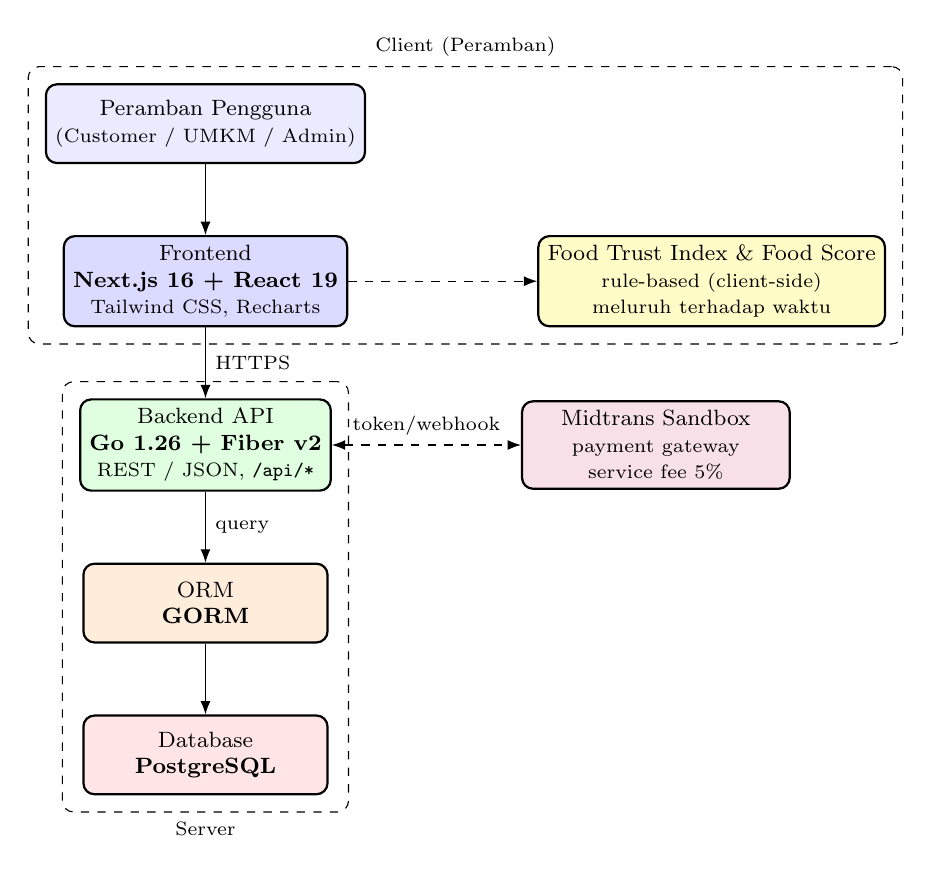
\begin{tikzpicture}[
    font=\footnotesize,
    layer/.style={rounded corners, draw, thick, minimum width=3.1cm, minimum height=1cm, align=center},
    node distance=0.9cm and 1.2cm,
]
% Client layer
\node[layer, fill=blue!8] (browser) {Peramban Pengguna\\\scriptsize(Customer / UMKM / Admin)};
\node[layer, fill=blue!14, below=of browser] (front) {Frontend\\\textbf{Next.js 16 + React 19}\\\scriptsize Tailwind CSS, Recharts};
\node[layer, fill=green!12, below=of front] (api) {Backend API\\\textbf{Go 1.26 + Fiber v2}\\\scriptsize REST / JSON, \texttt{/api/*}};
\node[layer, fill=orange!14, below=of api] (orm) {ORM\\\textbf{GORM}};
\node[layer, fill=red!10, below=of orm] (db) {Database\\\textbf{PostgreSQL}};

% Food Score annotation (client-side rule-based)
\node[layer, fill=yellow!22, right=2.4cm of front, minimum width=3.4cm] (score) {Food Trust Index \& Food Score\\\scriptsize rule-based (client-side)\\\scriptsize meluruh terhadap waktu};

% External payment gateway
\node[layer, fill=purple!12, right=2.4cm of api, minimum width=3.4cm] (pay) {Midtrans Sandbox\\\scriptsize payment gateway\\\scriptsize service fee 5\%};

\draw[-{Latex}] (browser) -- (front);
\draw[-{Latex}] (front) -- node[right]{\scriptsize HTTPS} (api);
\draw[-{Latex}] (api) -- node[right]{\scriptsize query} (orm);
\draw[-{Latex}] (orm) -- (db);
\draw[-{Latex}, dashed] (front) -- (score);
\draw[{Latex}-{Latex}, dashed] (api) -- node[above, font=\scriptsize]{token/webhook} (pay);

\begin{scope}[on background layer]
    \node[draw, dashed, rounded corners, fit=(browser)(front)(score), inner sep=6pt, label={[font=\scriptsize]above:Client (Peramban)}] {};
    \node[draw, dashed, rounded corners, fit=(api)(orm)(db), inner sep=6pt, label={[font=\scriptsize]below:Server}] {};
\end{scope}
\end{tikzpicture}
\caption{Arsitektur High-Level Savora}
\label{fig:arsitektur}
\end{figure}

Alur komunikasi sistem:
\begin{enumerate}[leftmargin=*]
    \item \textbf{Client Layer} : Peramban pengguna menjalankan aplikasi Next.js/React. Food Score dihitung di sisi klien secara \textit{rule-based} dan diperbarui mengikuti sisa waktu rescue.
    \item \textbf{Application Layer} : \textit{Request} diteruskan ke backend Go/Fiber melalui REST API (\texttt{/api/*}) yang memproses \textit{business logic} produk, pesanan, analitik, dan iklan.
    \item \textbf{Payment Gateway} : Untuk pembayaran \textit{cashless}, backend membuat token transaksi ke Midtrans \textit{sandbox} dan memperbarui status order setelah memverifikasi notifikasi/\textit{webhook}.
    \item \textbf{Data Access Layer} : GORM memetakan model ke tabel dan menjalankan kueri ke database.
    \item \textbf{Data Layer} : PostgreSQL menyimpan data persisten (UMKM, produk, pesanan, ulasan, iklan, pembayaran).
\end{enumerate}

\bigskip

% ==================== BAGIAN 8: BATASAN PERANGKAT LUNAK ====================
\section{RUANG LINGKUP DAN BATASAN PERANGKAT LUNAK}

Bagian ini mendefinisikan ruang lingkup \textit{Minimum Viable Product} (MVP) Savora, yaitu
batas fungsionalitas yang menjadi fokus pengembangan untuk lomba CODE 6.0. Ruang lingkup ini
mengacu pada dokumen kebutuhan produk (PRD) Savora dan diposisikan sebagai rancangan MVP yang
dapat diprototipekan dan diuji, bukan klaim bisnis yang sudah berjalan penuh.

\subsection{Ruang Lingkup MVP (In-Scope)}

Fungsionalitas berikut termasuk dalam ruang lingkup MVP Savora. Untuk transparansi, status
implementasi ditandai sebagai \emph{sudah berjalan} (telah ada pada basis kode) atau
\emph{direncanakan} (menjadi bagian MVP dan sedang/akan diimplementasikan).

\begin{enumerate}[leftmargin=*]
    \item \textbf{Autentikasi dan Manajemen Role} : Registrasi dan login untuk empat peran ---
    Customer, UMKM, Admin, dan Mitra Donasi --- dengan \textit{role-based access control}.

    \item \textbf{Manajemen Produk UMKM} : UMKM menambah, mengubah, dan menghapus produk makanan
    surplus (produk reguler maupun \textit{mystery box}) lengkap dengan harga asli, harga rescue,
    stok, foto, alamat pickup, dan batas waktu (\textit{expires\_at}).

    \item \textbf{Food Trust Index} : Penilaian kelayakan berbasis aturan dari input UMKM
    (kategori, jam produksi, metode penyimpanan, kondisi kemasan) yang menghasilkan lima status
    kelayakan dan menentukan apakah produk dapat dipublikasikan.

    \item \textbf{Food Score Decay} : Skor kelayakan (0--100) yang meluruh mengikuti sisa waktu
    rescue menuju \textit{expired}, ditampilkan \textit{real-time} beserta \textit{rescue timer}.

    \item \textbf{Keyword Classification dari Ulasan} : Klasifikasi keyword ulasan ke level
    Aman/Warning/Gawat dan akumulasi menjadi badge keamanan per UMKM.

    \item \textbf{Marketplace Customer} : Konsumen menelusuri produk rescue aktif, melihat Food
    Score, harga rescue, persentase diskon, dan badge keyword, serta menyaring dan mengurutkan produk.

    \item \textbf{Checkout Cashless via Midtrans} : Pembayaran \textit{cashless only} melalui Midtrans
    \textit{sandbox} dengan \textit{service fee} 5\% otomatis, pembuatan \textit{pickup code} setelah
    status \textit{Paid}, dan reservasi stok berbatas waktu.

    \item \textbf{Manajemen Pesanan dan Pickup} : Pencatatan pesanan dan siklus status (Created,
    Payment Pending, Paid, Ready for Pickup, Completed, No-Show, dll.) serta validasi \textit{pickup
    code} oleh UMKM.

    \item \textbf{Dashboard Analitik \& Insight UMKM} : Ringkasan penjualan, produk terlaris, tren,
    metrik listing (views, CTR, \textit{conversion rate}), serta \textit{insight} rating dan keyword.

    \item \textbf{Slot Iklan} : UMKM memasang iklan produk (paket berdurasi tetap) dan pihak ketiga
    dapat beriklan; seluruhnya melalui \textit{approval} admin.

    \item \textbf{Ulasan dan Rating} : Konsumen memberi rating dan ulasan dengan input keyword
    setelah transaksi selesai.

    \item \textbf{Help Center} : Customer melaporkan kendala (produk tidak tersedia/tidak sesuai,
    UMKM tidak merespons, masalah pembayaran) untuk ditangani admin.

    \item \textbf{Waste Log} : UMKM mencatat makanan tidak layak/tidak terjual sebagai bahan
    evaluasi produksi.

    \item \textbf{Konsol Admin} : Verifikasi UMKM, verifikasi Mitra Donasi (\textit{approve/reject}),
    moderasi listing dan iklan, dashboard keuangan (\textit{service fee} + iklan), dan \textit{export}
    laporan (CSV/Excel/PDF).

    \item \textbf{Mitra Donasi} : Registrasi organisasi non-profit dan verifikasi oleh admin untuk
    menerima makanan surplus.
\end{enumerate}

\subsection{Status Implementasi Fitur MVP}

Tabel~\ref{tab:mvp_scope} merangkum ruang lingkup MVP beserta status implementasi saat proposal ini
disusun. Fitur berstatus \emph{Sudah berjalan} telah tersedia pada basis kode (\textit{frontend}
Next.js dan/atau \textit{backend} Go/Fiber), sedangkan \emph{Direncanakan} merupakan bagian MVP yang
sedang/akan diselesaikan dalam \textit{sprint} berikutnya.

\begin{table}[htbp]
\centering
\caption{Ringkasan Ruang Lingkup dan Status MVP}
\label{tab:mvp_scope}
\small
\begin{tabularx}{\textwidth}{|>{\RaggedRight\arraybackslash}p{0.32\textwidth}|l|>{\RaggedRight\arraybackslash}X|}
\hline
\textbf{Fitur MVP} & \textbf{Status} & \textbf{Keterangan} \\
\hline
Manajemen produk UMKM & Sudah berjalan & CRUD produk reguler \& \textit{mystery box} \\
\hline
Food Score Decay & Sudah berjalan & Rule-based, meluruh terhadap waktu (\textit{frontend}) \\
\hline
Keyword classification ulasan & Sudah berjalan & Level Aman/Warning/Gawat (\textit{frontend}) \\
\hline
Marketplace customer & Sudah berjalan & Browse, filter, sort, Food Score live \\
\hline
Manajemen pesanan & Sudah berjalan & Pencatatan \& update status \\
\hline
Dashboard analitik \& insight UMKM & Sudah berjalan & Penjualan, tren, insight, metrik listing \\
\hline
Slot iklan UMKM & Sudah berjalan & Paket iklan berdurasi tetap \\
\hline
Ulasan \& rating & Sudah berjalan & Dengan input keyword \\
\hline
Autentikasi \& role (4 peran) & Direncanakan & JWT + \textit{password hashing}, RBAC \\
\hline
Food Trust Index (input UMKM) & Direncanakan & Form penilaian $\rightarrow$ 5 status kelayakan \\
\hline
Checkout cashless Midtrans + \textit{service fee} 5\% & Direncanakan & Midtrans \textit{sandbox}, \textit{webhook}, \textit{pickup code} \\
\hline
Help Center & Direncanakan & Tiket bantuan customer $\rightarrow$ admin \\
\hline
Waste Log & Direncanakan & Pencatatan makanan tidak terjual \\
\hline
Konsol admin \& keuangan & Direncanakan & Verifikasi, moderasi, revenue, \textit{export} \\
\hline
Mitra Donasi & Direncanakan & Registrasi + verifikasi admin \\
\hline
\end{tabularx}
\end{table}

\subsection{Di Luar Ruang Lingkup MVP (Out-of-Scope)}

Kapabilitas berikut secara sadar dikeluarkan dari MVP dan diposisikan sebagai \textit{roadmap}
pengembangan lanjutan setelah MVP tervalidasi:

\begin{itemize}[leftmargin=*]
    \item Mode \textit{production} Midtrans dan perluasan kanal pembayaran (MVP menggunakan
    \textit{sandbox} saja; tidak ada pembayaran tunai/COD).
    \item Layanan \textit{delivery}/pengantaran (MVP hanya \textit{self-pickup}).
    \item \textit{Dynamic pricing} otomatis dan prediksi permintaan berbasis \textit{machine learning}
    (MVP menyediakan rekomendasi diskon \textit{rule-based}, harga akhir ditetapkan UMKM).
    \item Pengelolaan limbah eksternal (MVP membatasi pada pencatatan internal via \textit{Waste Log}).
    \item Komunikasi \textit{real-time} (\textit{push notification}, \textit{websocket}) dan aplikasi
    \textit{native mobile}.
    \item Voucher/promo dan integrasi POS UMKM.
\end{itemize}

\subsection{Asumsi dan Batasan}

\begin{itemize}[leftmargin=*]
    \item Aplikasi berbasis web \textit{responsive}/PWA-ready dan diakses melalui peramban modern
    (\textit{mobile-first}), bukan aplikasi \textit{native}.
    \item Food Trust Index dan Food Score merupakan indikator kelayakan berbasis aturan dan input
    UMKM, bukan hasil uji laboratorium; keputusan akhir konsumsi tetap pada pengguna.
    \item Integrasi Midtrans menggunakan mode \textit{sandbox} untuk demo dan pengujian, bukan
    transaksi uang asli.
    \item Estimasi dampak lingkungan (makanan terselamatkan, emisi) bersifat estimatif untuk edukasi,
    bukan klaim terverifikasi pihak ketiga.
    \item Data UMKM, customer, produk, dan transaksi dapat menggunakan \textit{dummy data} realistis
    untuk keperluan demonstrasi dan pengujian.
    \item Role Mitra Donasi pada MVP terbatas pada registrasi dan verifikasi oleh admin.
\end{itemize}

\bigskip

% ==================== BAGIAN 9: METODOLOGI PENGEMBANGAN ====================
\section{METODOLOGI PENGEMBANGAN}

\subsection{Metodologi yang Dipilih}

Savora dikembangkan menggunakan pendekatan \textbf{Agile/Scrum sederhana} dengan iterasi
\textit{sprint} pendek. Metodologi ini dipilih karena durasi lomba yang terbatas menuntut tim
melakukan iterasi cepat, membagi pekerjaan ke dalam \textit{sprint}, melakukan evaluasi harian,
dan memprioritaskan fitur MVP agar produk selaras dengan kebutuhan pengguna dan RuleBook lomba.

\subsection{Alasan Pemilihan Scrum}

\begin{enumerate}[leftmargin=*]
    \item \textbf{Iterasi Cepat} : Memungkinkan pengembangan dan pengujian fitur secara bertahap, sehingga bug dapat teridentifikasi lebih awal.
    \item \textbf{Feedback Berkala} : Stakeholder dapat memberikan masukan setiap akhir sprint untuk perbaikan berkelanjutan.
    \item \textbf{Transparansi} : Daily standup dan sprint review memastikan seluruh tim memiliki pemahaman yang sama tentang progres.
    \item \textbf{Adaptif} : Perubahan prioritas atau kebutuhan dapat diakomodasi tanpa mengganggu seluruh roadmap.
\end{enumerate}

\subsection{Tahapan dan Timeline Pengembangan}

Pengembangan Savora dijalankan dalam lima tahapan utama yang dipetakan ke dalam timeline lomba
selama 22 hari (4--25 Juli 2026).

\begin{table}[htbp]
\centering
\caption{Tahapan Pengembangan Savora}
\label{tab:tahapan}
\begin{tabularx}{\textwidth}{|l|X|X|}
\hline
\textbf{Tahap} & \textbf{Fokus} & \textbf{Output} \\
\hline
Discovery \& Scope Lock & Menentukan masalah, fitur, \textit{user flow}, dan batasan MVP & PRD final dan \textit{backlog} \\
\hline
Design Sprint & Wireframe, \textit{design system}, dan prototipe & Figma dan \textit{design spec} \\
\hline
Development Sprint & Implementasi \textit{frontend}, \textit{backend}, database, dan integrasi API & MVP berjalan \textit{end-to-end} \\
\hline
Testing \& Refinement & Pengujian, \textit{bug fixing}, dan perbaikan UX & Demo stabil \\
\hline
Submission Preparation & Proposal, video demo, deployment, dan README & Paket \textit{submission} lengkap \\
\hline
\end{tabularx}
\end{table}

\begin{table}[htbp]
\centering
\caption{Timeline 22 Hari Pengembangan Savora}
\label{tab:timeline}
\begin{tabularx}{\textwidth}{|l|l|X|}
\hline
\textbf{Minggu} & \textbf{Tanggal} & \textbf{Fokus dan Deliverable} \\
\hline
W1 & 4--10 Jul & Setup repo, database, \textit{auth}, API \textit{skeleton}, dan \textit{design system} \\
\hline
W2 & 11--17 Jul & Fitur inti: marketplace, Food Trust Index, pembayaran Midtrans, Help Center, Waste Log \\
\hline
W3 & 18--22 Jul & Dashboard, rating, analitik, \textit{testing}, deploy, dan video demo \\
\hline
Deadline & 25 Jul & \textit{Submission}: proposal PDF, video, GitHub, dan aplikasi \textit{deployed} \\
\hline
\end{tabularx}
\end{table}

\begin{figure}[htbp]
\centering
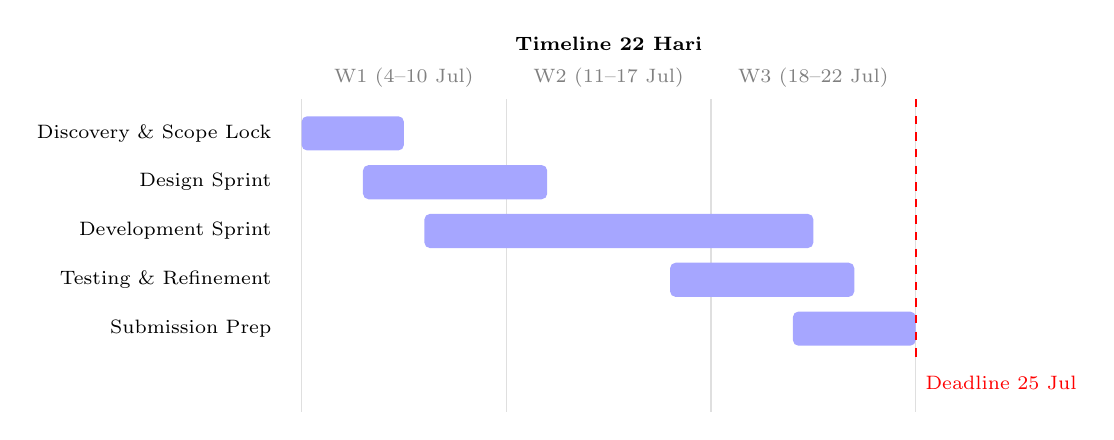
\begin{tikzpicture}[font=\scriptsize, x=2.6cm, y=0.62cm]
    % Grid minggu (3 kolom = W1, W2, W3)
    \foreach \w in {0,1,2,3} {
        \draw[gray!25] (\w,0.2) -- (\w,-6.2);
    }
    % Label minggu
    \foreach \w/\lbl in {0/{W1 (4--10 Jul)}, 1/{W2 (11--17 Jul)}, 2/{W3 (18--22 Jul)}} {
        \node[above, gray] at (\w+0.5, 0.25) {\lbl};
    }
    \node[above] at (1.5, 1.0) {\textbf{Timeline 22 Hari}};
    % Bar tahap: {row}{start}{len}{label}
    \foreach \row/\start/\len/\lbl in {
        0/0/0.5/{Discovery \& Scope Lock},
        1/0.3/0.9/{Design Sprint},
        2/0.6/1.9/{Development Sprint},
        3/1.8/0.9/{Testing \& Refinement},
        4/2.4/0.6/{Submission Prep}
    } {
        \fill[blue!35, rounded corners=2pt] (\start, -\row-0.15) rectangle (\start+\len, -\row-0.85);
        \node[left, black] at (-0.1, -\row-0.5) {\lbl};
    }
    % Milestone deadline
    \draw[red, thick, dashed] (3,0.2) -- (3,-5.2);
    \node[right, red, font=\scriptsize] at (3, -5.6) {Deadline 25 Jul};
\end{tikzpicture}
\caption{Timeline (Gantt Chart) Pengembangan Savora}
\label{fig:gantt}
\end{figure}

\subsection{Peran Anggota Tim}

\begin{table}[htbp]
\centering
\caption{Pembagian Tugas Anggota Tim}
\label{tab:peran}
\begin{tabularx}{\textwidth}{|l|Y|Y|}
\hline
\textbf{Anggota} & \textbf{Role} & \textbf{Tanggung Jawab} \\
\hline
Wa Ode Nur Alia & Auth, Admin, Keuangan, Mitra Donasi, Iklan & \textit{Auth} \& \textit{role} user, dashboard admin, keuangan platform, verifikasi mitra donasi, manajemen iklan, \textit{export} laporan \\
\hline
Richard Firmansyah & Marketplace Customer, Detail Produk, Slot Iklan & Beranda Food Score/Rescue Time, badge keyword safety, slot iklan marketplace, detail produk \\
\hline
Muhammad Rifaidi & Dashboard UMKM, Analitik, Insight, Iklan UMKM & Dashboard UMKM, analitik penjualan, \textit{insight} rating \& keyword, analitik pelacakan, pengiklanan produk \\
\hline
Ridwan Hakim Ramadhan & Food Score Decay, Keyword Classification & Rumus Food Score \textit{decay}, mesin klasifikasi keyword ulasan, API \textit{score} \& keyword \\
\hline
Nadi Azzada Akbar & Cashless, Service Fee, Order, Review Keyword & Sistem \textit{cashless} Midtrans, \textit{service fee} 5\%, checkout, \textit{order tracking}, input review keyword \\
\hline
\end{tabularx}
\end{table}

\subsection{Tools Pendukung}

\begin{itemize}[leftmargin=*]
    \item \textbf{Project Management} : Notion atau Trello untuk sprint board dan task tracking
    \item \textbf{Communication} : Discord atau WhatsApp Group untuk komunikasi harian
    \item \textbf{Design} : Figma untuk wireframe dan UI design
    \item \textbf{Documentation} : Google Docs untuk dokumentasi teknis
    \item \textbf{Version Control} : Git dengan branch strategy (main, develop, feature branches)
\end{itemize}

\bigskip

% ==================== BAGIAN 10: ARSITEKTUR SISTEM & DESAIN ====================
\section{ARSITEKTUR SISTEM}

\subsection{Use Case Diagram}

Terdapat empat aktor utama dalam sistem Savora, yaitu Customer, UMKM, Admin, dan Mitra Donasi.
Gambar~\ref{fig:usecase} memetakan use case utama per aktor sesuai ruang lingkup MVP.

\begin{figure}[htbp]
\centering
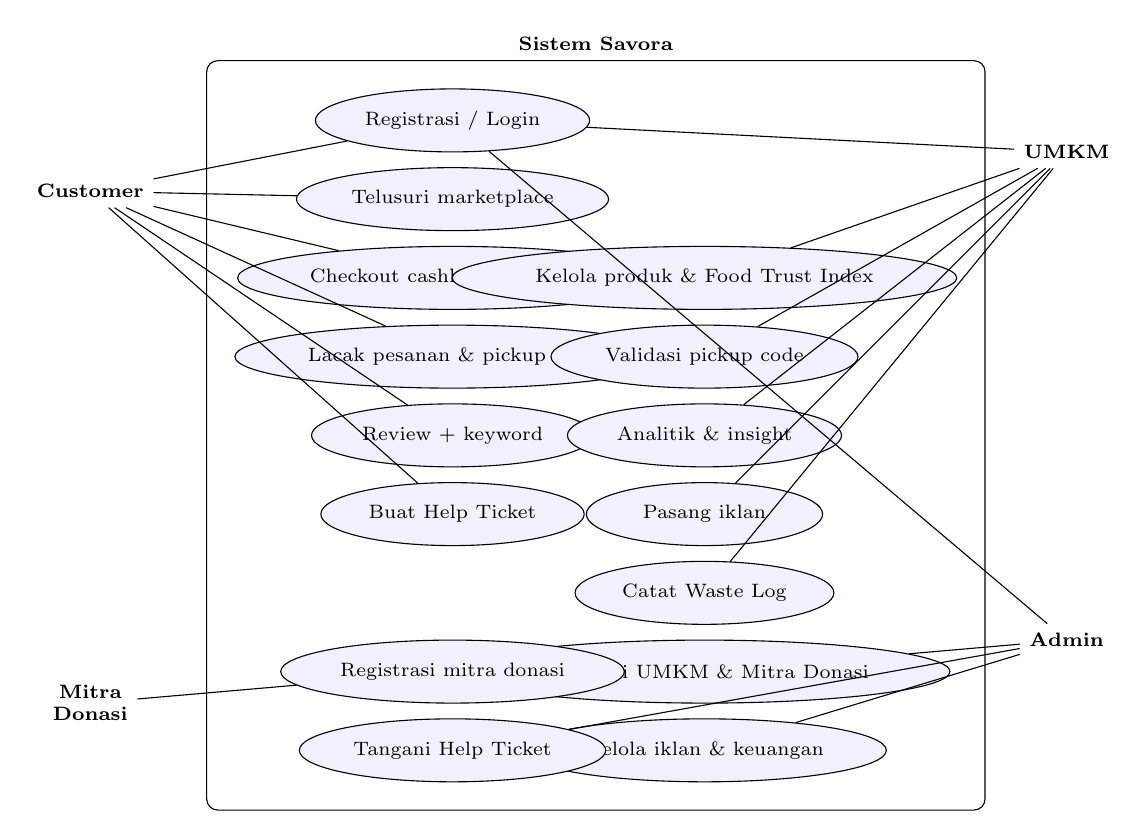
\begin{tikzpicture}[
    font=\scriptsize,
    actor/.style={align=center, font=\scriptsize\bfseries},
    uc/.style={draw, ellipse, minimum width=3.0cm, minimum height=0.8cm, align=center, fill=blue!6},
    node distance=0.3cm,
]
% Actors (left: customer/mitra, right: umkm/admin)
\node[actor] (cust)  at (0,0.5) {Customer};
\node[actor] (mitra) at (0,-6.0) {Mitra\\Donasi};
\node[actor] (umkm)  at (12.4,1.0) {UMKM};
\node[actor] (admin) at (12.4,-5.2) {Admin};

% Customer use cases
\node[uc] (uc1) at (4.6, 1.4) {Registrasi / Login};
\node[uc] (uc2) at (4.6, 0.4) {Telusuri marketplace};
\node[uc] (uc3) at (4.6,-0.6) {Checkout cashless (Midtrans)};
\node[uc] (uc4) at (4.6,-1.6) {Lacak pesanan \& pickup code};
\node[uc] (uc5) at (4.6,-2.6) {Review + keyword};
\node[uc] (uc6) at (4.6,-3.6) {Buat Help Ticket};
% UMKM use cases
\node[uc] (uc7) at (7.8,-0.6) {Kelola produk \& Food Trust Index};
\node[uc] (uc8) at (7.8,-1.6) {Validasi pickup code};
\node[uc] (uc9) at (7.8,-2.6) {Analitik \& insight};
\node[uc] (uc10) at (7.8,-3.6) {Pasang iklan};
\node[uc] (uc11) at (7.8,-4.6) {Catat Waste Log};
% Admin use cases
\node[uc] (uc12) at (7.8,-5.6) {Verifikasi UMKM \& Mitra Donasi};
\node[uc] (uc13) at (7.8,-6.6) {Kelola iklan \& keuangan};
\node[uc] (uc14) at (4.6,-6.6) {Tangani Help Ticket};
% Mitra donasi
\node[uc] (uc15) at (4.6,-5.6) {Registrasi mitra donasi};

% Customer links
\foreach \u in {uc1,uc2,uc3,uc4,uc5,uc6} \draw (cust) -- (\u);
% Mitra links
\draw (mitra) -- (uc15);
% UMKM links
\foreach \u in {uc1,uc7,uc8,uc9,uc10,uc11} \draw (umkm) -- (\u);
% Admin links
\foreach \u in {uc1,uc12,uc13,uc14} \draw (admin) -- (\u);

\begin{scope}[on background layer]
    \node[draw, rounded corners, fit=(uc1)(uc2)(uc3)(uc4)(uc5)(uc6)(uc7)(uc8)(uc9)(uc10)(uc11)(uc12)(uc13)(uc14)(uc15), inner sep=10pt, label={above:\textbf{Sistem Savora}}] {};
\end{scope}
\end{tikzpicture}
\caption{Use Case Diagram Savora (4 Aktor)}
\label{fig:usecase}
\end{figure}

\begin{enumerate}[leftmargin=*]
    \item \textbf{Customer} : Registrasi/login, menelusuri marketplace (Food Score, rescue timer, badge keyword), checkout \textit{cashless} via Midtrans, melacak pesanan dan \textit{pickup code}, memberi review dengan keyword, dan membuat \textit{Help Ticket}.
    \item \textbf{UMKM} : Mengelola produk beserta input Food Trust Index, memvalidasi \textit{pickup code}, memantau analitik dan \textit{insight}, memasang iklan, dan mencatat Waste Log.
    \item \textbf{Admin} : Memverifikasi UMKM dan Mitra Donasi, mengelola iklan dan keuangan platform (\textit{service fee} + iklan), serta menangani \textit{Help Ticket}.
    \item \textbf{Mitra Donasi} : Organisasi non-profit yang mendaftar dan menunggu verifikasi admin untuk menerima makanan surplus.
\end{enumerate}

\subsection{ERD (Entity Relationship Diagram)}

ERD pada Gambar~\ref{fig:erd} menampilkan entitas inti model data Savora sesuai PRD. Untuk menjaga
keterbacaan, diagram memuat entitas utama; daftar lengkap entitas beserta deskripsinya dirangkum
pada Tabel~\ref{tab:database}.

\begin{figure}[htbp]
\centering
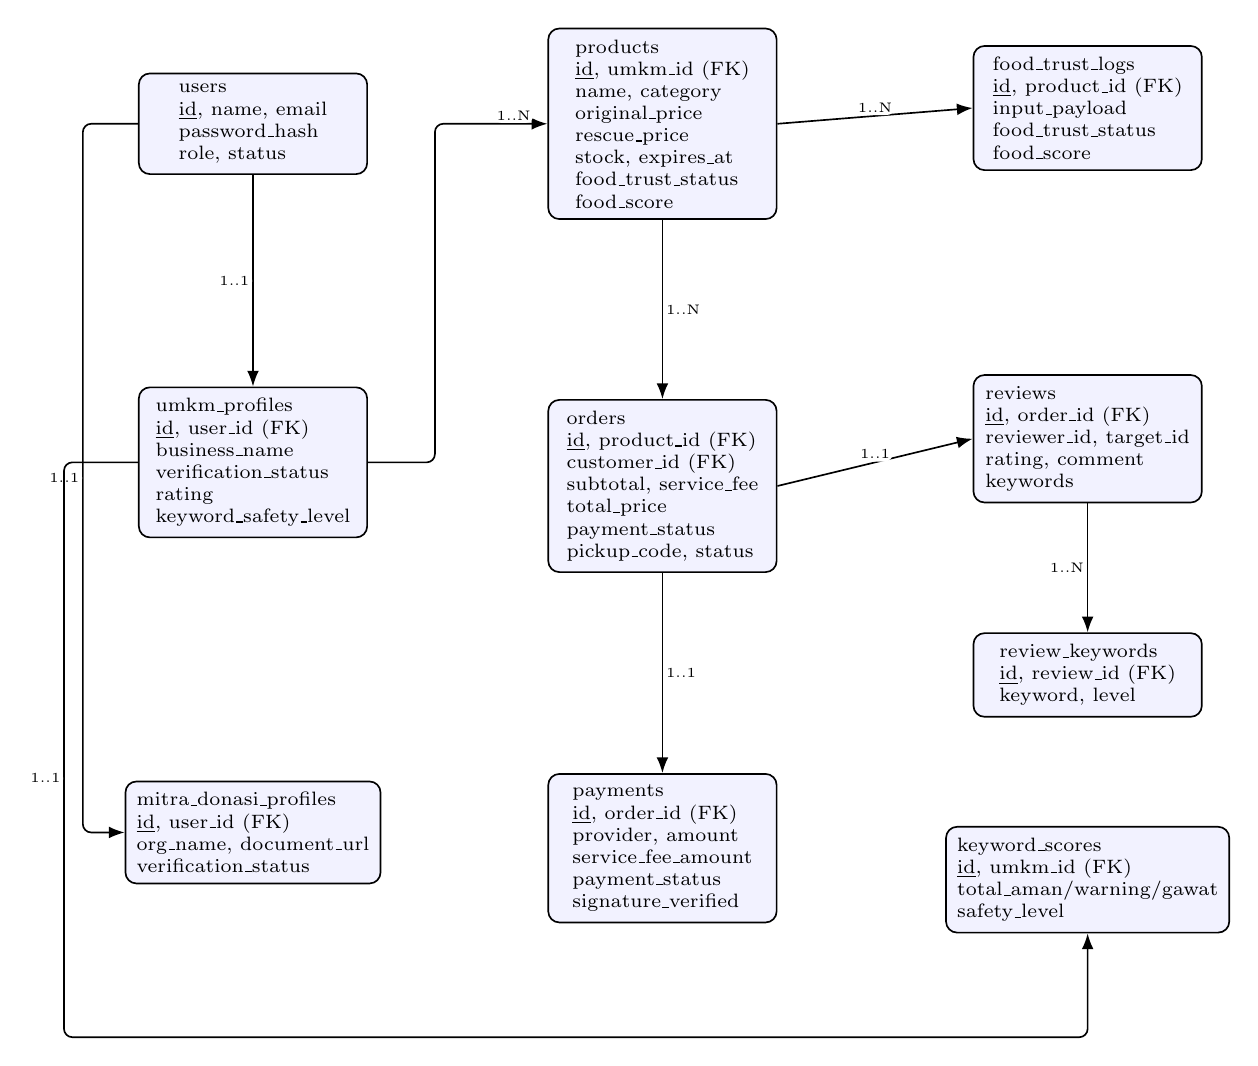
\begin{tikzpicture}[
    font=\scriptsize,
    entity/.style={draw, semithick, rounded corners, align=left, fill=blue!5,
                   inner sep=4pt, minimum width=2.9cm},
    ehead/.style={font=\scriptsize\bfseries},
    rel/.style={-{Latex[length=2mm]}, semithick, rounded corners=3pt},
    card/.style={font=\tiny, fill=white, inner sep=1pt},
]
% ---- Three tidy columns; rows aligned on a grid ----
% Column x-positions
\def\cxA{0}    % identitas / aktor
\def\cxB{5.2}  % transaksi
\def\cxC{10.6} % penilaian
% Column A: users, umkm_profiles, mitra_donasi_profiles
\node[entity] (user)  at (\cxA, 0)     {\ehead{users}\\ \underline{id}, name, email\\ password\_hash\\ role, status};
\node[entity] (umkm)  at (\cxA,-4.3)   {\ehead{umkm\_profiles}\\ \underline{id}, user\_id (FK)\\ business\_name\\ verification\_status\\ rating\\ keyword\_safety\_level};
\node[entity] (mitra) at (\cxA,-9.0)   {\ehead{mitra\_donasi\_profiles}\\ \underline{id}, user\_id (FK)\\ org\_name, document\_url\\ verification\_status};
% Column B: products -> orders -> payments
\node[entity] (prod)  at (\cxB, 0)     {\ehead{products}\\ \underline{id}, umkm\_id (FK)\\ name, category\\ original\_price\\ rescue\_price\\ stock, expires\_at\\ food\_trust\_status\\ food\_score};
\node[entity] (order) at (\cxB,-4.6)   {\ehead{orders}\\ \underline{id}, product\_id (FK)\\ customer\_id (FK)\\ subtotal, service\_fee\\ total\_price\\ payment\_status\\ pickup\_code, status};
\node[entity] (pay)   at (\cxB,-9.2)   {\ehead{payments}\\ \underline{id}, order\_id (FK)\\ provider, amount\\ service\_fee\_amount\\ payment\_status\\ signature\_verified};
% Column C: logs / reviews / keywords / scores
\node[entity] (ftl)   at (\cxC, 0.2)   {\ehead{food\_trust\_logs}\\ \underline{id}, product\_id (FK)\\ input\_payload\\ food\_trust\_status\\ food\_score};
\node[entity] (review)at (\cxC,-4.0)   {\ehead{reviews}\\ \underline{id}, order\_id (FK)\\ reviewer\_id, target\_id\\ rating, comment\\ keywords};
\node[entity] (kw)    at (\cxC,-7.0)   {\ehead{review\_keywords}\\ \underline{id}, review\_id (FK)\\ keyword, level};
\node[entity] (ks)    at (\cxC,-9.6)   {\ehead{keyword\_scores}\\ \underline{id}, umkm\_id (FK)\\ total\_aman/warning/gawat\\ safety\_level};

% ---- Orthogonal relationship routing (no crossing / sloped labels) ----
% users --< umkm_profiles (1..1), straight vertical in column A
\draw[rel] (user.south)  -- node[card,left]{1..1} (umkm.north);
% users --< mitra_donasi_profiles (1..1): orthogonal route down the left margin
\draw[rel] (user.west) -- ++(-0.7,0) |- node[card,pos=0.25,left]{1..1} (mitra.west);
% umkm_profiles --< products (1..N): out-right into the column gap, then up to products' left side
\draw[rel] (umkm.east) -- ++(0.85,0) |- node[card,pos=0.85,above]{1..N} (prod.west);
% products --< orders (1..N), straight vertical in column B
\draw[rel] (prod.south)  -- node[card,right]{1..N} (order.north);
% orders --< payments (1..1), straight vertical in column B
\draw[rel] (order.south) -- node[card,right]{1..1} (pay.north);
% products --< food_trust_logs (1..N), horizontal B->C at top row
\draw[rel] (prod.east)   -- node[card,above]{1..N} (ftl.west);
% orders --< reviews (1..1), horizontal B->C
\draw[rel] (order.east)  -- node[card,above]{1..1} (review.west);
% reviews --< review_keywords (1..N), straight vertical in column C
\draw[rel] (review.south)-- node[card,left]{1..N} (kw.north);
% umkm_profiles --< keyword_scores (1..1): routed below all boxes, no overlap
\draw[rel] (umkm.west) -- (-2.4,-4.3)
           -- (-2.4,-11.6) node[card,pos=0.55,left]{1..1}
           -- (\cxC,-11.6) -- (ks.south);
\end{tikzpicture}
\caption{Entity Relationship Diagram Savora (Entitas Inti)}
\label{fig:erd}
\end{figure}

\subsubsection{Daftar Entitas Data}

\begin{table}[htbp]
\centering
\caption{Struktur Data Model Savora}
\label{tab:database}
\small
\begin{tabularx}{\textwidth}{|l|X|}
\hline
\textbf{Entitas} & \textbf{Deskripsi} \\
\hline
users & Akun pengguna (role: Customer, UMKM, Admin, Mitra Donasi), status, kredensial \\
\hline
customer\_profiles & Profil customer: telepon, alamat, avatar \\
\hline
umkm\_profiles & Profil UMKM: nama usaha, lokasi, status verifikasi, rating, level keamanan keyword \\
\hline
mitra\_donasi\_profiles & Profil mitra donasi: nama organisasi, dokumen legalitas, status verifikasi \\
\hline
products & Produk surplus: harga asli/rescue, stok, batas waktu, status \& skor kelayakan \\
\hline
food\_trust\_logs & Riwayat perhitungan Food Trust Index per produk (input, status, skor) \\
\hline
orders & Pesanan: subtotal, service fee, total, metode \& status pembayaran, pickup code, status \\
\hline
payments & Transaksi Midtrans: provider, jumlah, service fee, status, verifikasi signature \\
\hline
reviews & Rating dan ulasan customer beserta keyword \\
\hline
review\_keywords & Keyword hasil klasifikasi ulasan dan level (Aman/Warning/Gawat) \\
\hline
keyword\_scores & Akumulasi keyword per UMKM dan level keamanan agregat \\
\hline
advertisements & Iklan UMKM/pihak ketiga: judul, durasi, harga, service fee, status approval \\
\hline
ad\_metrics / umkm\_analytics & Metrik iklan dan analitik UMKM (impressions, CTR, conversion, AOV) \\
\hline
platform\_revenue & Catatan pendapatan platform (service fee + iklan) \\
\hline
help\_tickets & Tiket bantuan customer: kategori, deskripsi, bukti, status, catatan admin \\
\hline
waste\_logs & Catatan makanan tidak layak/tidak terjual (kategori, berat, alasan, foto) \\
\hline
notifications / audit\_logs & Notifikasi pengguna dan log audit aksi admin \\
\hline
\end{tabularx}
\end{table}

\subsection{API Design}

Backend Go/Fiber mengekspos REST API berformat JSON. Tabel~\ref{tab:api} merangkum endpoint utama
sesuai rancangan MVP. Endpoint yang telah tersedia pada basis kode ditandai kolom Status
\emph{Ada}, sedangkan endpoint yang menjadi bagian MVP dan direncanakan ditandai \emph{Rencana}.

\begin{table}[htbp]
\centering
\caption{Endpoint API Utama}
\label{tab:api}
\small
\begin{tabularx}{\textwidth}{|l|>{\RaggedRight\arraybackslash}p{0.30\textwidth}|X|l|}
\hline
\textbf{Method} & \textbf{Endpoint} & \textbf{Deskripsi} & \textbf{Status} \\
\hline
POST & /auth/register, /auth/login & Registrasi \& login (4 role) & Rencana \\
\hline
GET & /products/marketplace & Daftar produk rescue aktif & Ada \\
\hline
POST/PUT/DELETE & /products, /products/:id & Kelola produk UMKM & Ada \\
\hline
POST & /food-trust/calculate & Hitung Food Trust Index & Rencana \\
\hline
POST & /orders & Buat order cashless via Midtrans & Rencana \\
\hline
POST & /payments/midtrans-token & Buat token pembayaran Midtrans sandbox & Rencana \\
\hline
POST & /payments/midtrans-webhook & Terima \& verifikasi notifikasi pembayaran & Rencana \\
\hline
PUT & /orders/:id/status & Update status pesanan & Ada \\
\hline
POST & /orders/:id/validate-pickup & Validasi pickup code & Rencana \\
\hline
POST & /reviews, GET /reviews/keywords/:umkm\_id & Review + keyword safety per UMKM & Rencana \\
\hline
POST/GET & /help-tickets & Buat \& kelola tiket bantuan & Rencana \\
\hline
POST/GET & /waste-logs & Catat \& lihat Waste Log & Rencana \\
\hline
GET & /analytics/dashboard/:umkm\_id, /insight, /top-products & Analitik \& insight UMKM & Ada \\
\hline
POST/GET/PUT & /ads, /ads/active, /ads/:id/status & Kelola \& tayangkan iklan & Ada \\
\hline
POST & /mitra-donasi/register & Registrasi mitra donasi & Rencana \\
\hline
PATCH & /admin/mitra-donasi/:id/verify & Verifikasi mitra donasi & Rencana \\
\hline
GET & /admin/revenue, /admin/revenue/export & Keuangan platform \& export laporan & Rencana \\
\hline
\end{tabularx}
\end{table}

\subsection{Alur Data}

\subsubsection{Alur Penjualan Savora}
Gambar~\ref{fig:alur_jual} menggambarkan alur utama \textit{food rescue} pada Savora, dari pemuatan
produk oleh UMKM hingga ulasan oleh customer. Warna kotak menandai pelaku: biru untuk UMKM, oranye
untuk proses sistem, dan hijau untuk customer. Harga rescue ditetapkan UMKM, sedangkan Food Score
dihitung sistem dan meluruh mengikuti sisa waktu.

\begin{figure}[htbp]
\centering
\begin{tikzpicture}[
    font=\scriptsize,
    step/.style={draw, semithick, rounded corners, align=center,
                 minimum height=1.35cm, text width=3.1cm, inner sep=4pt},
    umkm/.style={step, fill=blue!8},
    sys/.style={step, fill=orange!12},
    cust/.style={step, fill=green!10},
    num/.style={circle, draw, fill=white, inner sep=1pt, font=\scriptsize\bfseries},
    flow/.style={-{Latex[length=2.6mm]}, semithick},
]
% Grid: 3 kolom x 3 baris (susunan boustrophedon) supaya garis alur jelas
\def\cA{0}\def\cB{5.3}\def\cC{10.6}
\def\rA{0}\def\rB{-3.0}\def\rC{-6.0}
% Baris 1 (kiri -> kanan): langkah 1,2,3
\node[umkm] (a) at (\cA,\rA) {UMKM \emph{upload} produk + set harga \emph{rescue}};
\node[sys]  (b) at (\cB,\rA) {Sistem hitung Food Score (\emph{decay})};
\node[sys]  (c) at (\cC,\rA) {Produk tampil di \emph{marketplace}};
% Baris 2 (kanan -> kiri): langkah 4,5,6
\node[cust] (d) at (\cC,\rB) {Customer telusuri \& \emph{checkout cashless}};
\node[umkm] (e) at (\cB,\rB) {UMKM proses status pesanan};
\node[cust] (f) at (\cA,\rB) {\emph{Self-pickup} + validasi \emph{pickup code}};
% Baris 3 (kiri -> kanan): langkah 7,8
\node[cust] (g) at (\cA,\rC) {Customer beri \emph{rating} \& ulasan};
\node[sys]  (h) at (\cB,\rC) {\emph{Update} keyword safety \& analitik};
% Nomor langkah
\foreach \n/\bx in {1/a,2/b,3/c,4/d,5/e,6/f,7/g,8/h}
    \node[num] at (\bx.north west) {\n};
% Alur: baris1 (L->R) -> turun -> baris2 (R->L) -> turun -> baris3 (L->R)
\draw[flow] (a) -- (b);
\draw[flow] (b) -- (c);
\draw[flow] (c) -- (d);   % turun di kolom kanan
\draw[flow] (d) -- (e);
\draw[flow] (e) -- (f);
\draw[flow] (f) -- (g);   % turun di kolom kiri
\draw[flow] (g) -- (h);
\end{tikzpicture}
\caption{Alur Penjualan Savora}
\label{fig:alur_jual}
\end{figure}

\subsubsection{Alur Pembayaran Cashless dan Status Pesanan}
Pembayaran Savora bersifat \textit{cashless} melalui Midtrans \textit{sandbox}. Gambar~\ref{fig:alur_bayar}
menggambarkan transisi status pesanan dari pembuatan order hingga selesai atau gagal. Stok
di-reserve saat \textit{Payment Pending} dan dikembalikan bila pembayaran gagal/kedaluwarsa;
\textit{pickup code} dibuat setelah status \textit{Paid}.

\begin{figure}[htbp]
\centering
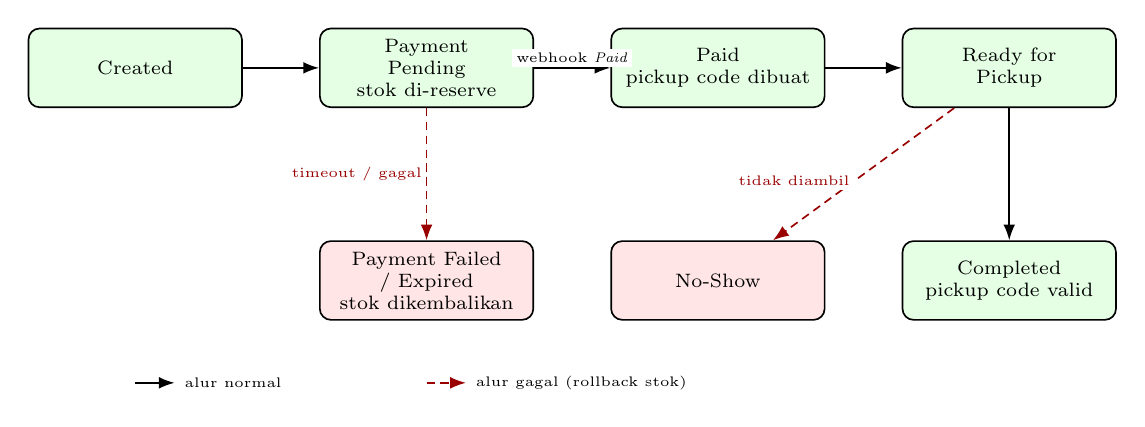
\begin{tikzpicture}[
    font=\scriptsize,
    st/.style={draw, semithick, rounded corners, fill=green!10, align=center,
               minimum height=1.0cm, text width=2.5cm, inner sep=3pt},
    bad/.style={draw, semithick, rounded corners, fill=red!10, align=center,
                minimum height=1.0cm, text width=2.5cm, inner sep=3pt},
    lbl/.style={font=\tiny, fill=white, inner sep=1.5pt, midway},
    flow/.style={-{Latex[length=2mm]}, semithick},
    badflow/.style={-{Latex[length=2mm]}, semithick, red!60!black, densely dashed},
]
% Grid: happy path on top row (y=0), failure states on bottom row (y=-2.6)
% Generous horizontal gap (3.6cm) so edge labels never touch boxes.
\node[st] (created) at (0,0)     {Created};
\node[st] (pending) at (3.7,0)   {Payment\\Pending\\\scriptsize stok di-reserve};
\node[st] (paid)    at (7.4,0)   {Paid\\\scriptsize pickup code dibuat};
\node[st] (ready)   at (11.1,0)  {Ready for\\Pickup};
\node[st] (done)    at (11.1,-2.7){Completed\\\scriptsize pickup code valid};
% Failure states on the bottom row, clear of the happy-path labels
\node[bad] (fail)   at (3.7,-2.7) {Payment Failed\\/ Expired\\\scriptsize stok dikembalikan};
\node[bad] (noshow) at (7.4,-2.7) {No-Show};

% Happy path (horizontal), labels sit on the arrow with white background
\draw[flow] (created) -- (pending);
\draw[flow] (pending) -- node[lbl,above]{webhook \textit{Paid}} (paid);
\draw[flow] (paid)    -- (ready);
\draw[flow] (ready)   -- (done);
% Failure transitions (dashed, downward) with labels beside the arrow
\draw[badflow] (pending) -- node[lbl,left]{timeout / gagal} (fail);
\draw[badflow] (ready)   -- node[lbl,left,pos=0.55]{tidak diambil} (noshow);
% Legend (drawn directly on canvas, no nested tikzpicture)
\draw[flow] (0,-4.0) -- ++(0.5,0) node[right, font=\tiny, black]{alur normal};
\draw[badflow] (3.7,-4.0) -- ++(0.5,0) node[right, font=\tiny, black]{alur gagal (rollback stok)};
\end{tikzpicture}
\caption{Alur Status Pesanan dan Pembayaran Cashless}
\label{fig:alur_bayar}
\end{figure}

\subsubsection{Alur Iklan UMKM}
Sesuai layanan iklan aplikasi, sebuah iklan berpindah status \textbf{Draft} $\rightarrow$
\textbf{Aktif} $\rightarrow$ \textbf{Kadaluarsa}, di mana status kadaluarsa dihitung dari tanggal
akhir tayang (\texttt{end\_at}).

\begin{figure}[htbp]
\centering
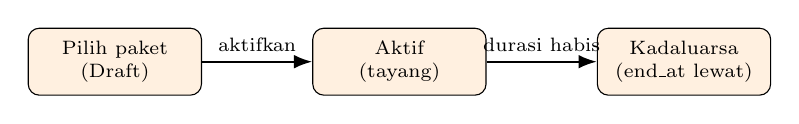
\begin{tikzpicture}[
    font=\scriptsize, node distance=1.4cm,
    st/.style={draw, rounded corners, fill=orange!12, minimum width=2.2cm, minimum height=0.85cm, align=center},
    flow/.style={-{Latex}, thick},
]
\node[st] (draft) {Pilih paket\\(Draft)};
\node[st, right=of draft] (active) {Aktif\\\scriptsize (tayang)};
\node[st, right=of active] (exp) {Kadaluarsa\\\scriptsize (end\_at lewat)};
\draw[flow] (draft) -- node[above]{aktifkan} (active);
\draw[flow] (active) -- node[above]{durasi habis} (exp);
\end{tikzpicture}
\caption{Alur Status Iklan UMKM}
\label{fig:alur_iklan}
\end{figure}

\subsubsection{Alur Admin dan Mitra Donasi}
Admin mengakses dashboard untuk memantau statistik platform, memverifikasi UMKM dan Mitra Donasi
(\textit{approve}/\textit{reject} berdasarkan dokumen legalitas), memoderasi listing dan iklan,
menangani \textit{Help Ticket}, serta melihat dashboard keuangan (\textit{service fee} + iklan) dan
melakukan \textit{export} laporan. Mitra Donasi mendaftar melalui halaman registrasi dan berstatus
\emph{pending} hingga diverifikasi admin.

\bigskip

% ==================== BAGIAN 11: IMPLEMENTASI TEKNIS ====================
\section{ALGORITMA DAN LOGIKA APLIKASI}

Bab ini menjelaskan logika inti Savora: \textit{Food Trust Index} (penilaian kelayakan berbasis
input UMKM), \textit{Food Score Decay} (skor kelayakan yang meluruh terhadap waktu), \textit{Keyword
Classification} (klasifikasi keamanan dari ulasan), \textit{Dynamic Discount} (rekomendasi diskon),
serta perhitungan \textit{service fee} pada pembayaran \textit{cashless}. Seluruh logika dirancang
\textit{rule-based} (deterministik) sehingga transparan, \textit{explainable}, dapat diaudit, dan
dapat dihitung \textit{real-time} tanpa layanan \textit{machine learning} terpisah.

\subsection{Prioritas Implementasi Fitur}

Tabel~\ref{tab:implementasi} merangkum status implementasi fitur utama, konsisten dengan ruang
lingkup MVP (lihat bab Ruang Lingkup dan Batasan Perangkat Lunak).

\begin{table}[htbp]
\centering
\caption{Status Implementasi Fitur}
\label{tab:implementasi}
\small
\begin{tabularx}{\textwidth}{|l|X|l|}
\hline
\textbf{Modul} & \textbf{Fitur} & \textbf{Status} \\
\hline
\multirow{6}{*}{UMKM} & Kelola produk (reguler \& mystery box) & Sudah berjalan \\
\cline{2-3}
& Food Score Decay & Sudah berjalan \\
\cline{2-3}
& Dashboard analitik \& insight & Sudah berjalan \\
\cline{2-3}
& Iklan produk & Sudah berjalan \\
\cline{2-3}
& Kelola status pesanan & Sudah berjalan \\
\cline{2-3}
& Food Trust Index (input UMKM) \& Waste Log & Direncanakan \\
\hline
\multirow{4}{*}{Customer} & Marketplace \& Food Score live & Sudah berjalan \\
\cline{2-3}
& Keyword classification ulasan & Sudah berjalan \\
\cline{2-3}
& Checkout cashless (Midtrans) + service fee 5\% & Direncanakan \\
\cline{2-3}
& Pesanan, pickup code, Help Center & Direncanakan \\
\hline
\multirow{2}{*}{Auth} & Login / Register (4 role) & Direncanakan \\
\cline{2-3}
& Role-based access & Direncanakan \\
\hline
Admin & Verifikasi UMKM/Mitra Donasi, keuangan, moderasi & Direncanakan \\
\hline
\multirow{2}{*}{Lanjutan} & Dynamic pricing otomatis (ML) & Roadmap \\
\cline{2-3}
& Prediksi permintaan (ML), real-time & Roadmap \\
\hline
\end{tabularx}
\end{table}

\subsection{Food Trust Index}

Food Trust Index (FTI) adalah penilaian kelayakan makanan berbasis aturan yang dihitung dari input
UMKM saat membuat listing. FTI bersifat transparan dan \textit{explainable}, bukan sertifikasi
laboratorium, dan tidak menggantikan pemeriksaan langsung customer saat pickup.

\subsubsection{Input dan Output}

Input FTI meliputi kategori makanan, waktu masak/produksi, metode penyimpanan, kondisi kemasan, dan
ada/tidaknya kuah/saus. Berdasarkan akumulasi indikasi risiko dari input tersebut, sistem
memetakan produk ke salah satu dari lima status pada Tabel~\ref{tab:fti}.

\begin{table}[htbp]
\centering
\caption{Output Food Trust Index}
\label{tab:fti}
\small
\begin{tabularx}{\textwidth}{|l|X|l|}
\hline
\textbf{Status} & \textbf{Makna (berdasarkan input UMKM)} & \textbf{Aksi Sistem} \\
\hline
Fresh & Makanan baru, kemasan baik, penyimpanan sesuai & Publikasikan \\
\hline
Layak Dijual & Masih dalam estimasi masa simpan, tanpa indikasi risiko & Publikasikan \\
\hline
Segera Dijual & Mendekati batas waktu konsumsi, kemasan masih memadai & Publikasikan + urgency \& diskon tinggi \\
\hline
Tidak Disarankan Dijual & Indikasi risiko sedang (penyimpanan/waktu kurang ideal) & Tidak tampil; evaluasi internal \\
\hline
Tidak Layak Konsumsi & Indikasi risiko tinggi (lewat masa/kemasan buruk) & Tidak tampil; arahkan ke Waste Log \\
\hline
\end{tabularx}
\end{table}

\subsubsection{Aturan Penilaian}

Penilaian menggunakan pendekatan sederhana yang dapat dijelaskan ke juri: setiap indikator input
diberi bobot risiko; akumulasi risiko rendah menghasilkan status \emph{Fresh}/\emph{Layak Dijual},
risiko sedang menghasilkan \emph{Segera Dijual}/\emph{Tidak Disarankan Dijual}, dan risiko tinggi
menghasilkan \emph{Tidak Layak Konsumsi}. Setiap detail produk wajib menampilkan \textit{disclaimer}
bahwa FTI dihitung dari informasi UMKM dan aturan platform, dan customer tetap disarankan memeriksa
kondisi makanan saat pickup. Status FTI juga berperan sebagai skor awal/plafon ($S_0$) bagi
perhitungan Food Score Decay pada subbab berikut.

\subsection{Food Score Decay}

Food Score adalah indikator kelayakan makanan bernilai 0--100 yang menurun seiring
berkurangnya sisa waktu rescue menuju batas kedaluwarsa. Model ini mengacu pada konsep
\textit{freshness index} / masa simpan makanan \textit{perishable}: kesegaran cenderung bertahan
di awal masa simpan lalu turun lebih cepat menjelang batas layak konsumsi, sehingga kurvanya
sedikit konveks \cite{iotshelflife2025}.

\subsubsection{Rumus}

Misalkan $t_{r}$ adalah sisa waktu rescue, $W$ adalah lebar jendela rescue (nilai $t_{r}$ saat
produk pertama dimuat), dan $S_{0}$ adalah skor awal/plafon dari UMKM (mis. Food Trust Index,
maksimum 100). Fraksi kesegaran didefinisikan sebagai:

\begin{equation}
f = \frac{\max(0,\ \min(t_{r},\ W))}{W}, \qquad 0 \le f \le 1
\end{equation}

Food Score dihitung dengan peluruhan berpangkat (\textit{power decay}):

\begin{equation}
\mathrm{FES} = \operatorname{round}\!\left( S_{0} \cdot f^{\,\gamma} \right), \qquad \gamma = 0.65
\end{equation}

Eksponen $\gamma = 0.65$ ($<1$) membuat kurva konveks: skor bertahan relatif tinggi di awal dan
turun lebih tajam menjelang kedaluwarsa. Sebagai contoh, pada $S_{0}=100$: saat $f=0{,}5$ maka
$\mathrm{FES}\approx 64$, dan saat $f=0{,}2$ maka $\mathrm{FES}\approx 35$. Gambar~\ref{fig:decay}
menampilkan profil peluruhan tersebut.

\begin{figure}[htbp]
\centering
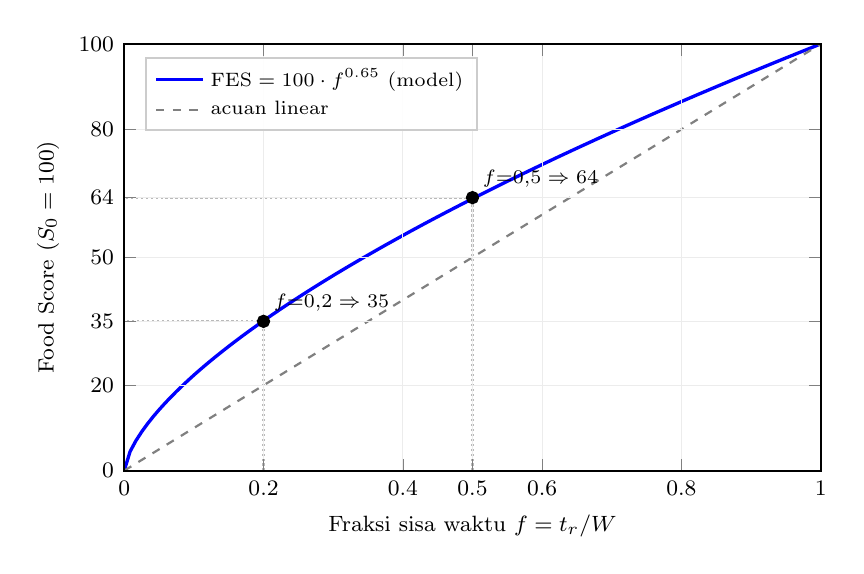
\begin{tikzpicture}
\begin{axis}[
    width=0.86\textwidth, height=7cm,
    xlabel={Fraksi sisa waktu $f = t_r / W$},
    ylabel={Food Score ($S_0=100$)},
    xmin=0, xmax=1, ymin=0, ymax=100,
    xtick={0,0.2,0.4,0.5,0.6,0.8,1},
    ytick={0,20,35,50,64,80,100},
    grid=both, grid style={gray!15}, minor tick num=0,
    domain=0:1, samples=120,
    thick, font=\footnotesize,
    legend pos=north west,
    legend cell align=left,
    legend style={draw=gray!40, font=\scriptsize, fill=white, fill opacity=0.9, text opacity=1},
    axis on top,
]
% Power-decay curve (the model)
\addplot[blue, very thick] {100*(x^0.65)};
\addlegendentry{$\mathrm{FES}=100\cdot f^{0.65}$ (model)}
% Linear reference for contrast
\addplot[gray, dashed, thick] {100*x};
\addlegendentry{acuan linear}
% Example points cited in the text, with guide lines and labels
\addplot[only marks, mark=*, mark size=2pt, black] coordinates {(0.5,64) (0.2,35)};
\draw[gray!55, densely dotted] (axis cs:0.5,0) -- (axis cs:0.5,64) -- (axis cs:0,64);
\draw[gray!55, densely dotted] (axis cs:0.2,0) -- (axis cs:0.2,35) -- (axis cs:0,35);
\node[anchor=south west, font=\scriptsize] at (axis cs:0.5,64) {$f{=}0{,}5\Rightarrow 64$};
\node[anchor=south west, font=\scriptsize] at (axis cs:0.2,35) {$f{=}0{,}2\Rightarrow 35$};
\end{axis}
\end{tikzpicture}
\caption{Kurva Peluruhan Food Score ($\gamma=0.65$): skor bertahan tinggi di awal lalu turun lebih tajam mendekati kedaluwarsa}
\label{fig:decay}
\end{figure}

\subsubsection{Band Skor}

Skor dipetakan ke band kelayakan yang tampil ke pengguna beserta warna statusnya, sesuai ambang
pada kode:

\begin{table}[htbp]
\centering
\caption{Band Food Score}
\label{tab:fes_band}
\small
\begin{tabularx}{\textwidth}{|l|l|X|}
\hline
\textbf{Rentang Skor} & \textbf{Label} & \textbf{Makna} \\
\hline
$\ge 80$ & Sangat Layak & Kualitas masih prima \\
\hline
$60$--$79$ & Layak & Aman dikonsumsi \\
\hline
$35$--$59$ & Segera Ambil & Disarankan segera diambil \\
\hline
$1$--$34$ & Kritis & Mendekati batas kelayakan \\
\hline
$0$ & Kedaluwarsa & Melewati batas rescue \\
\hline
\end{tabularx}
\end{table}

\subsubsection{Alur Perhitungan}

\begin{figure}[htbp]
\centering
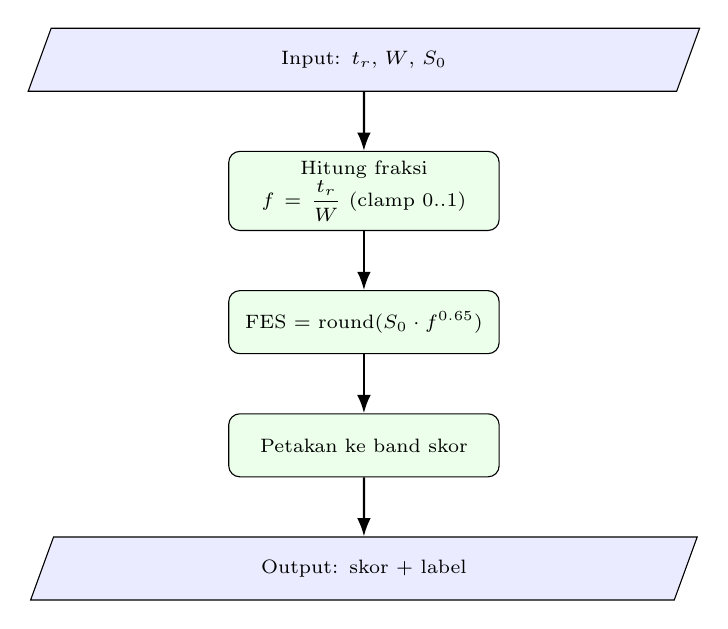
\begin{tikzpicture}[
    font=\scriptsize, node distance=0.75cm,
    io/.style={draw, trapezium, trapezium left angle=70, trapezium right angle=110, fill=blue!8, align=center, minimum height=0.8cm, text width=3.4cm, inner sep=2pt},
    proc/.style={draw, rounded corners, fill=green!8, align=center, minimum height=0.8cm, text width=3.2cm},
    dec/.style={draw, diamond, aspect=2, fill=orange!12, align=center, inner sep=1pt},
    flow/.style={-{Latex}, thick},
]
\node[io] (in) {Input: $t_r$, $W$, $S_0$};
\node[proc, below=of in] (frac) {Hitung fraksi $f=\dfrac{t_r}{W}$ (clamp $0..1$)};
\node[proc, below=of frac] (calc) {$\mathrm{FES}=\operatorname{round}(S_0\cdot f^{0.65})$};
\node[proc, below=of calc] (band) {Petakan ke band skor};
\node[io, below=of band] (out) {Output: skor + label};

\draw[flow] (in) -- (frac);
\draw[flow] (frac) -- (calc);
\draw[flow] (calc) -- (band);
\draw[flow] (band) -- (out);
\end{tikzpicture}
\caption{Flowchart Perhitungan Food Score}
\label{fig:fes_flow}
\end{figure}

\subsection{Keyword Classification dari Ulasan}

Selain rating numerik, Savora mengklasifikasikan keyword pada ulasan customer untuk membangun
sinyal keamanan makanan per UMKM secara \textit{crowdsourced}. Mesin klasifikasi bersifat
\textit{rule-based} dan telah tersedia pada basis kode (\textit{frontend}).

\subsubsection{Kamus dan Tingkat Keamanan}

Keyword dipetakan ke tiga tingkat keamanan dengan peringkat (\textit{rank}) berbeda, sebagaimana
Tabel~\ref{tab:keyword}. Jika sebuah ulasan memuat beberapa keyword sekaligus, tingkat paling gawat
yang menang (prinsip \textit{worst-case}).

\begin{table}[htbp]
\centering
\caption{Tingkat Keamanan Keyword Ulasan}
\label{tab:keyword}
\small
\begin{tabularx}{\textwidth}{|l|l|X|}
\hline
\textbf{Level} & \textbf{Rank} & \textbf{Contoh Keyword} \\
\hline
Gawat & 3 & basi, berjamur, busuk, beracun, keracunan, kadaluarsa \\
\hline
Warning & 2 & bau, asam, tengik, apek, lembek, kurang segar \\
\hline
Aman & 1 & enak, segar, fresh, lezat, bersih, higienis, gurih \\
\hline
\end{tabularx}
\end{table}

\subsubsection{Agregasi ke Badge UMKM}

Untuk setiap UMKM, sistem menghitung jumlah ulasan per level dan mengambil level terburuk yang
muncul sebagai badge keamanan (Aman/Warning/Gawat). Bila tersedia level yang telah dihitung
\textit{backend} (mis. via \texttt{keyword\_scores}), nilai tersebut diprioritaskan; jika tidak,
sistem melakukan agregasi lokal dari daftar ulasan. Badge ini ditampilkan pada kartu dan halaman
detail UMKM sehingga customer memperoleh sinyal keamanan tambahan sebelum bertransaksi.

\subsection{Dynamic Discount dan Perhitungan Harga}

Pada MVP, harga rescue ($p_{r}$) ditetapkan oleh UMKM saat membuat produk. Sistem memberikan
\emph{rekomendasi} rentang diskon berdasarkan status Food Trust Index (mis. \emph{Segera Dijual}
disarankan diskon 35--50\%), namun keputusan akhir tetap di tangan UMKM dengan \textit{guardrail}
harga minimum agar tetap menguntungkan (\textit{time-aware manual pricing}). Sistem kemudian
menghitung besaran diskon dan penghematan secara otomatis dari harga asli ($p_{o}$) dan harga
rescue tersebut.

\subsubsection{Rumus}

\begin{equation}
\mathrm{diskon}\ (\%) = \operatorname{round}\!\left( \frac{p_{o} - p_{r}}{p_{o}} \times 100 \right), \qquad p_o > 0
\end{equation}

\begin{equation}
\mathrm{penghematan} = p_{o} - p_{r}
\end{equation}

Nilai diskon di-\textit{clamp} agar tidak negatif. Diskon dan penghematan inilah yang ditampilkan
pada kartu produk di marketplace, berdampingan dengan Food Score dan \textit{countdown}
sisa waktu rescue.

\subsubsection{Alur Penetapan Harga}

\begin{figure}[htbp]
\centering
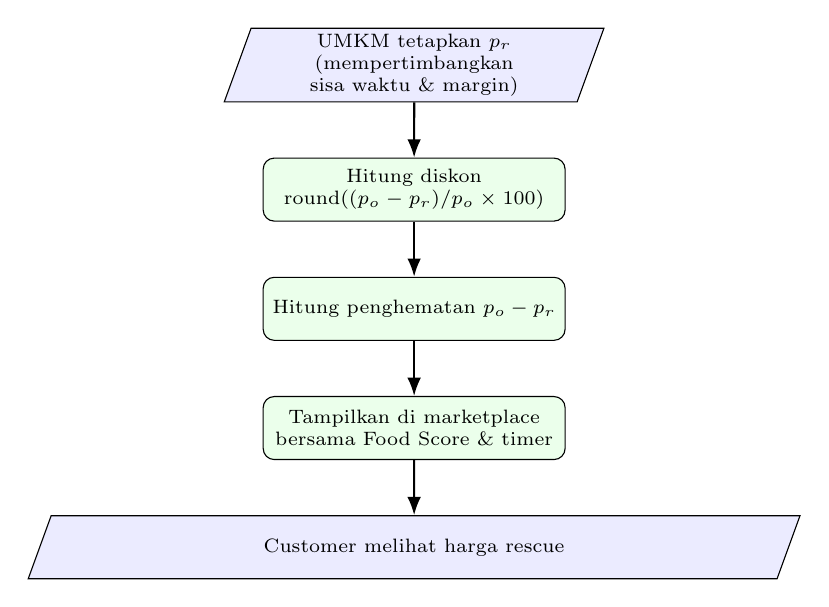
\begin{tikzpicture}[
    font=\scriptsize, node distance=0.7cm,
    io/.style={draw, trapezium, trapezium left angle=70, trapezium right angle=110, fill=blue!8, align=center, minimum height=0.8cm, text width=4cm, inner sep=2pt},
    proc/.style={draw, rounded corners, fill=green!8, align=center, minimum height=0.8cm, text width=3.6cm},
    flow/.style={-{Latex}, thick},
]
\node[io] (in) {UMKM tetapkan $p_r$ (mempertimbangkan sisa waktu \& margin)};
\node[proc, below=of in] (disc) {Hitung diskon\\$\operatorname{round}((p_o-p_r)/p_o\times100)$};
\node[proc, below=of disc] (save) {Hitung penghematan $p_o-p_r$};
\node[proc, below=of save] (show) {Tampilkan di marketplace bersama Food Score \& timer};
\node[io, below=of show] (out) {Customer melihat harga rescue};
\draw[flow] (in) -- (disc);
\draw[flow] (disc) -- (save);
\draw[flow] (save) -- (show);
\draw[flow] (show) -- (out);
\end{tikzpicture}
\caption{Flowchart Penetapan dan Perhitungan Harga Rescue}
\label{fig:pricing_flow}
\end{figure}

\subsubsection{Roadmap: Dynamic Pricing Otomatis}

Penetapan harga otomatis berbasis \textit{reinforcement learning} seperti \textit{Q-learning} untuk
meminimalkan food waste \cite{qlearning2026pricing} diposisikan sebagai pengembangan lanjutan
(\textit{out-of-scope} MVP). Pendekatan ini akan mengoptimalkan harga berdasarkan elastisitas
permintaan lokal dan sisa waktu kelayakan secara adaptif, menggantikan penetapan manual saat ini.

\subsection{Perhitungan Service Fee pada Pembayaran Cashless}

Model pendapatan utama Savora adalah \textit{service fee} 5\% per transaksi. Untuk sebuah pesanan
dengan subtotal produk $p_{r}$ (harga rescue $\times$ kuantitas), sistem menghitung:

\begin{equation}
\mathrm{service\_fee} = \operatorname{round}(0{,}05 \times \mathrm{subtotal}), \qquad
\mathrm{total} = \mathrm{subtotal} + \mathrm{service\_fee}
\end{equation}

Nilai \textit{service fee} dan total ditampilkan transparan di halaman checkout sebelum customer
membayar. Backend membuat token transaksi ke Midtrans \textit{sandbox} sebesar $\mathrm{total}$,
lalu memperbarui status pesanan menjadi \emph{Paid} hanya setelah menerima dan memverifikasi
notifikasi/\textit{signature} dari Midtrans. Setelah \emph{Paid}, sistem membuat \textit{pickup
code} unik untuk validasi pengambilan oleh UMKM, dan akumulasi \textit{service fee} dicatat pada
pendapatan platform (\texttt{platform\_revenue}).

\subsection{Integrasi Antar Komponen}
\begin{itemize}[leftmargin=*]
    \item \textbf{Frontend--Backend} : Komunikasi via RESTful API dengan format JSON.
    \item \textbf{Backend--Database} : Menggunakan GORM (ORM untuk Go) untuk akses PostgreSQL, termasuk \textit{auto-migration} skema.
    \item \textbf{Food Score} : Dihitung di sisi frontend secara \textit{rule-based} dan diperbarui \textit{real-time} mengikuti \textit{countdown} sisa waktu rescue.
    \item \textbf{Pembayaran} : Backend berkomunikasi dengan Midtrans \textit{sandbox} untuk membuat token transaksi dan memverifikasi notifikasi/\textit{webhook} sebelum memperbarui status order.
\end{itemize}

\bigskip

% ==================== BAGIAN 12: ANALISIS UI/UX & ACCESSIBILITY ====================
\section{RENCANA DESAIN UI/UX}

\subsection{Pendekatan User Research yang Akan Dilakukan}

Untuk memahami kebutuhan pengguna sebelum mulai implementasi, akan dilakukan penelitian sebagai berikut:

\begin{enumerate}[leftmargin=*]
    \item \textbf{Wawancara dengan UMKM Kuliner} : Akan dilakukan wawancara mendalam untuk memahami tantangan mereka dalam pengelolaan makanan surplus.
    
    \item \textbf{Survei Online} : Akan disebarkan kuesioner kepada konsumen potensial untuk mengetahui preferensi pembelian makanan surplus.
    
    \item \textbf{Observasi Lapangan} : Akan dilakukan pengamatan langsung terhadap operasional UMKM kuliner untuk mengidentifikasi pain points.
\end{enumerate}

\textbf{CATATAN}: Research ini akan dilakukan pada fase awal development, belum dilaksanakan saat ini.

\subsection{Target User Persona (Draft)}

\subsubsection{Persona 1: UMKM Kuliner (Draft)}
\begin{table}[htbp]
\centering
\begin{tabularx}{0.8\textwidth}{|l|X|}
\hline
\textbf{Aspek} & \textbf{Karakteristik} \\
\hline
Usia & 30-55 tahun \\
\hline
Usaha & Warung makan, kafe, katering \\
\hline
Teknologi & Cukup mahir menggunakan smartphone \\
\hline
Kebutuhan & Mengurangi food waste, menambah pendapatan \\
\hline
Pain Point & Kesulitan prediksi permintaan, tidak ada platform khusus \\
\hline
\end{tabularx}
\end{table}

\subsubsection{Persona 2: Customer (Draft)}
\begin{table}[htbp]
\centering
\begin{tabularx}{0.8\textwidth}{|l|X|}
\hline
\textbf{Aspek} & \textbf{Karakteristik} \\
\hline
Usia & 18-40 tahun (milenial dan Gen Z) \\
\hline
Pekerjaan & Mahasiswa, karyawan swasta \\
\hline
Kebutuhan & Makanan berkualitas dengan harga terjangkau \\
\hline
Pain Point & Ketidakyakinan terhadap kelayakan makanan diskon \\
\hline
\end{tabularx}
\end{table}

\subsubsection{Persona 3: Admin Platform (Draft)}
\begin{table}[htbp]
\centering
\begin{tabularx}{0.8\textwidth}{|l|X|}
\hline
\textbf{Aspek} & \textbf{Karakteristik} \\
\hline
Usia & 25-45 tahun \\
\hline
Peran & Operator platform, moderator \\
\hline
Kebutuhan & Monitoring transaksi, verifikasi UMKM \& Mitra Donasi, keuangan platform \\
\hline
\end{tabularx}
\end{table}

\subsubsection{Persona 4: Mitra Donasi (Draft)}
\begin{table}[htbp]
\centering
\begin{tabularx}{0.8\textwidth}{|l|X|}
\hline
\textbf{Aspek} & \textbf{Karakteristik} \\
\hline
Bentuk & Yayasan, panti, komunitas sosial, bank makanan \\
\hline
Peran & Menerima makanan surplus dari UMKM \\
\hline
Kebutuhan & Registrasi mudah, verifikasi legalitas, akses makanan surplus \\
\hline
Pain Point & Sulit menemukan sumber donasi makanan yang rutin dan tepercaya \\
\hline
\end{tabularx}
\end{table}

\subsection{Antarmuka Aplikasi (Prototipe)}

Prototipe antarmuka Savora telah dibangun dengan Next.js dan Tailwind CSS mengikuti prinsip
\textit{mobile-first} serta heuristik usability Nielsen \cite{nielsen2020heuristics}. Berikut
tangkapan layar dari halaman-halaman utama. Layar untuk alur \textit{cashless} (checkout Midtrans,
\textit{pickup code}), Help Center, Waste Log, serta registrasi/verifikasi Mitra Donasi merupakan
bagian MVP yang sedang diselesaikan dan dirangkum pada inventaris layar (Tabel~\ref{tab:screens}).

\subsubsection{Alur Customer}

\begin{figure}[htbp]
\centering
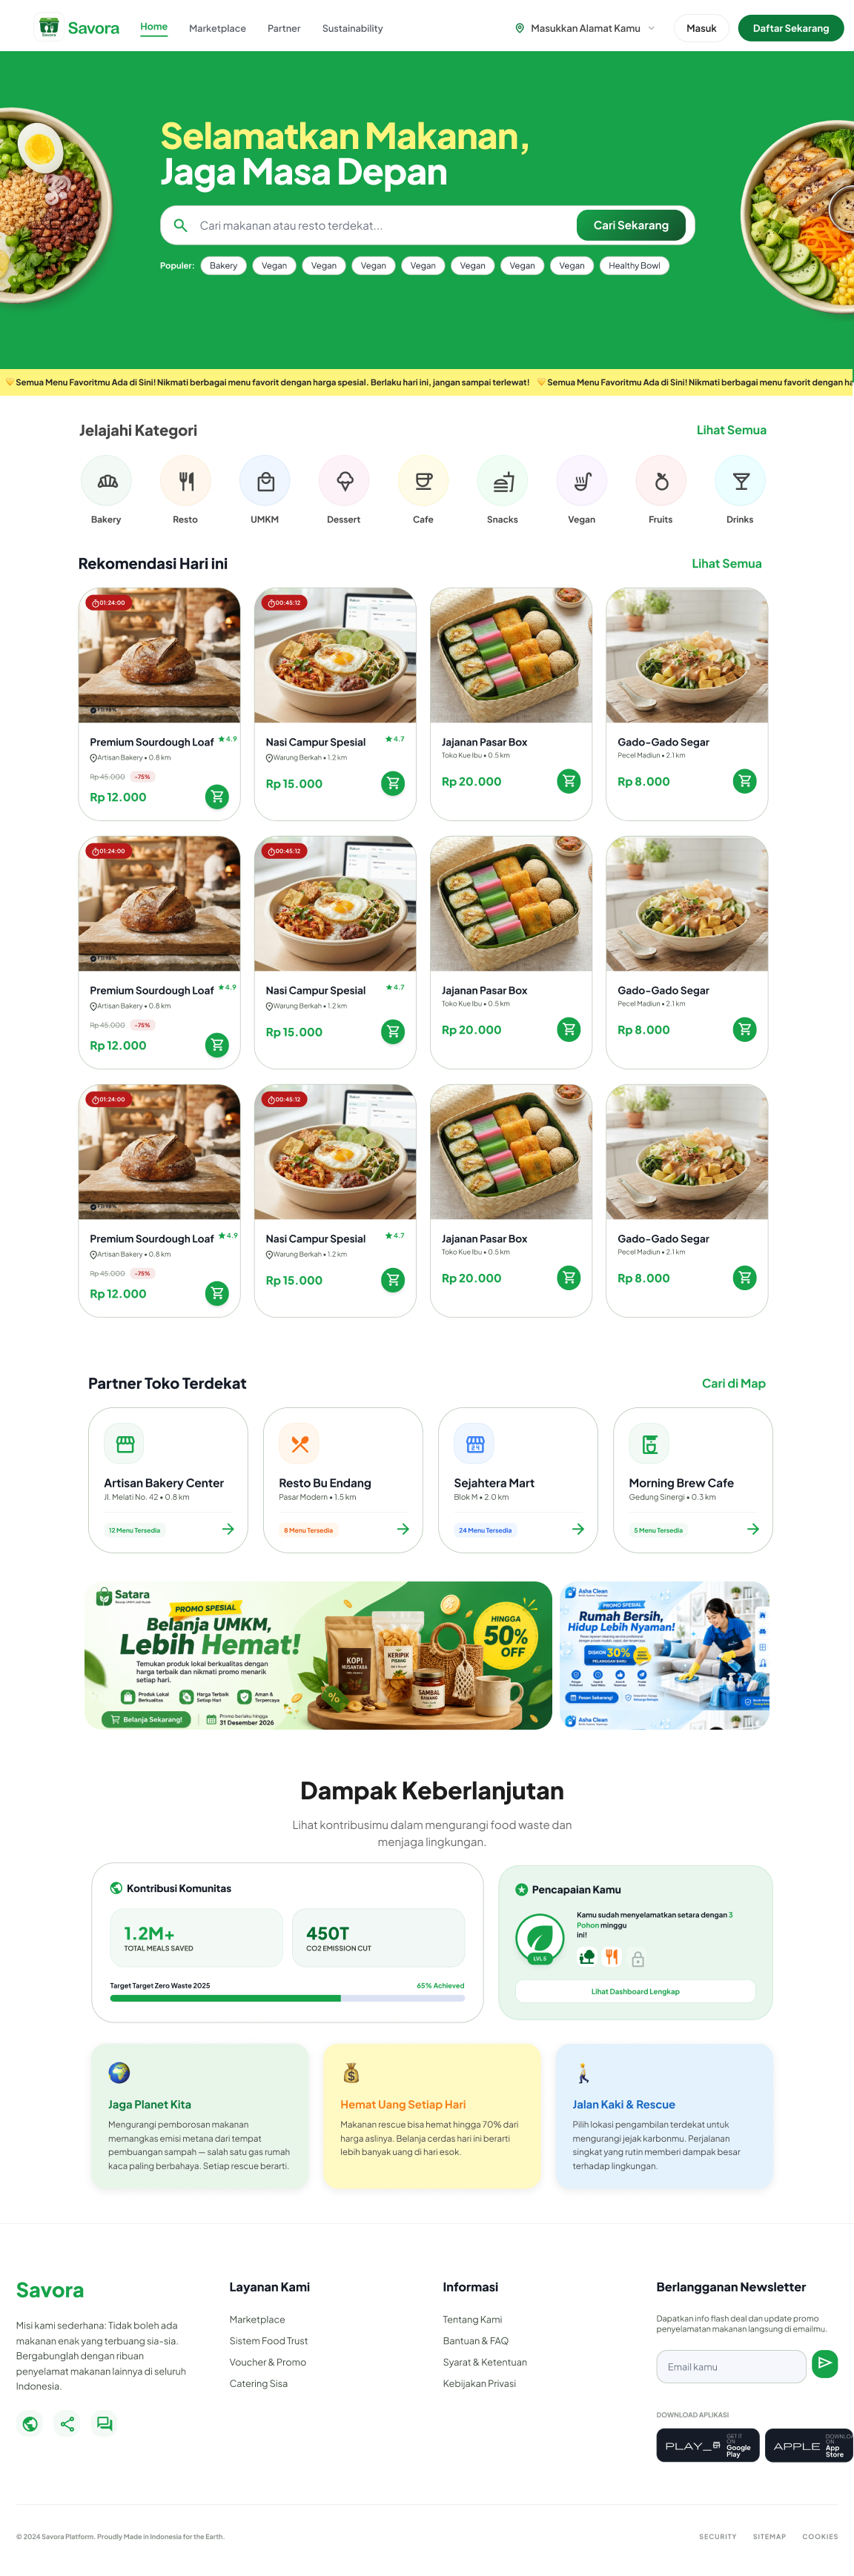
\includegraphics[width=0.74\textwidth, height=6.6cm, keepaspectratio]{gambar/beranda-customer.png}
\caption{Beranda / Marketplace Customer dengan Food Score dan timer rescue}
\label{fig:ui_beranda}
\end{figure}

\subsubsection{Alur UMKM}

% Dua dashboard UMKM disandingkan agar padat dan tidak menyisakan ruang kosong
\begin{figure}[htbp]
\centering
\begin{minipage}[t]{0.49\textwidth}
\centering
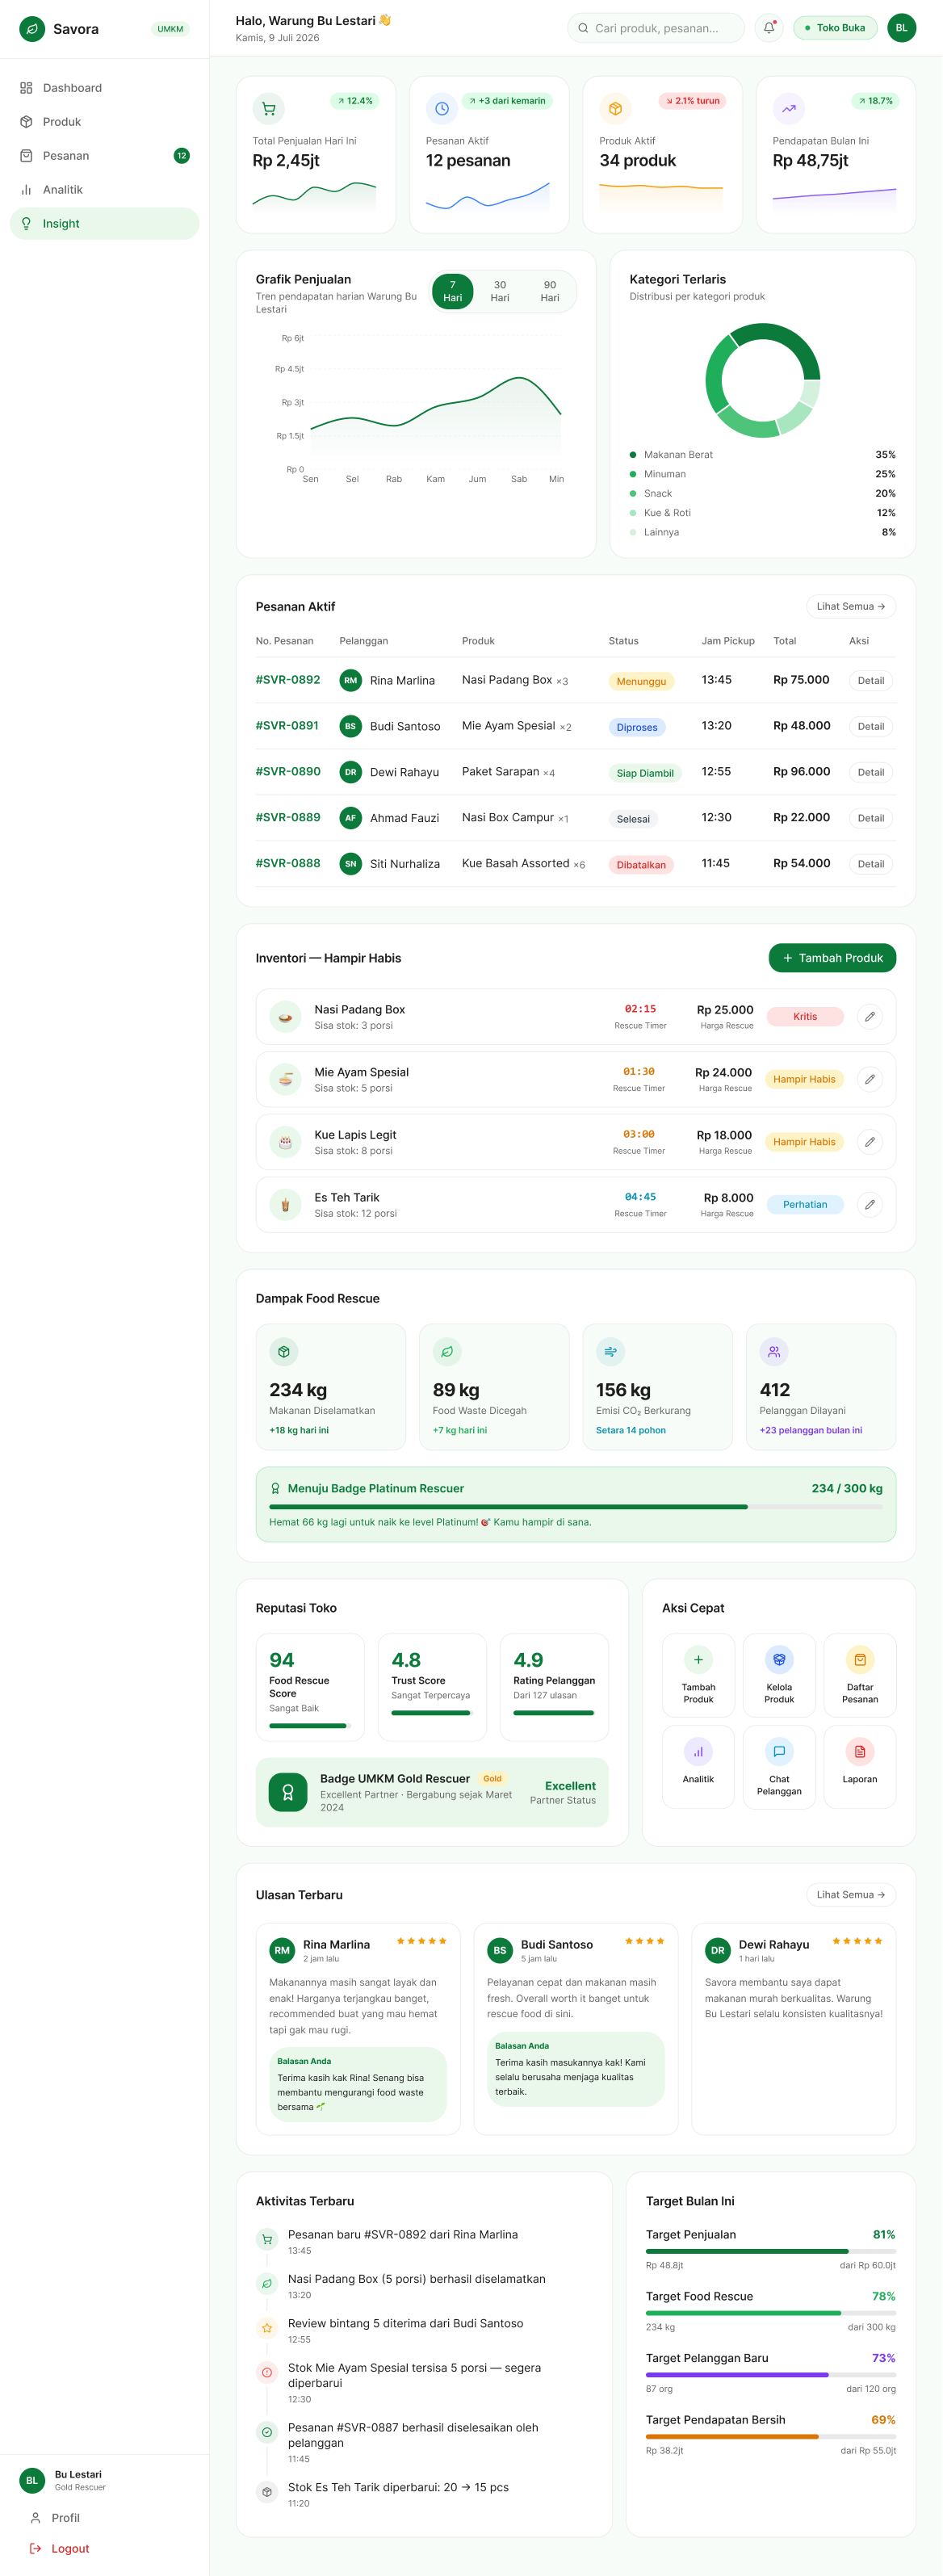
\includegraphics[width=\linewidth, height=5.2cm, keepaspectratio]{gambar/dashboard-umkm.png}
\caption{Dashboard UMKM}
\label{fig:ui_dashboard}
\end{minipage}\hfill
\begin{minipage}[t]{0.49\textwidth}
\centering
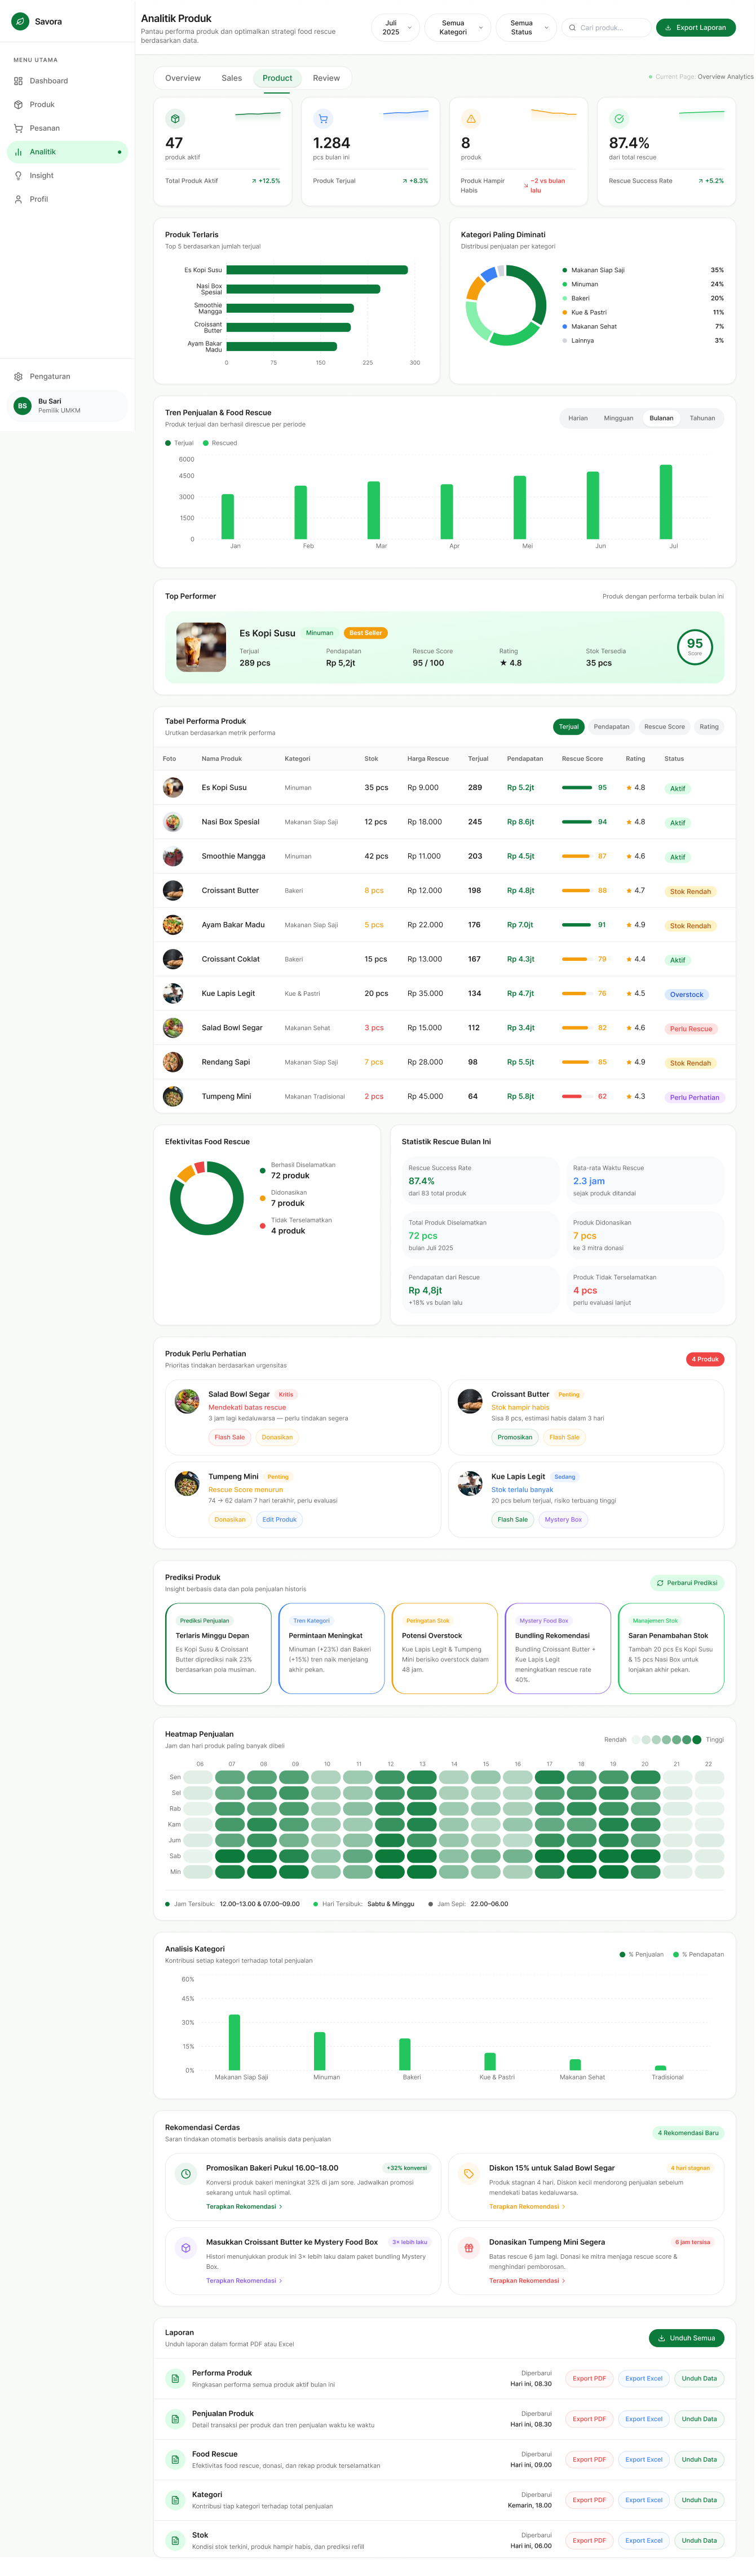
\includegraphics[width=\linewidth, height=5.2cm, keepaspectratio]{gambar/analitik-produk.png}
\caption{Analitik Produk UMKM}
\label{fig:ui_analitik}
\end{minipage}
\end{figure}

\begin{figure}[htbp]
\centering
\begin{minipage}[t]{0.49\textwidth}
\centering
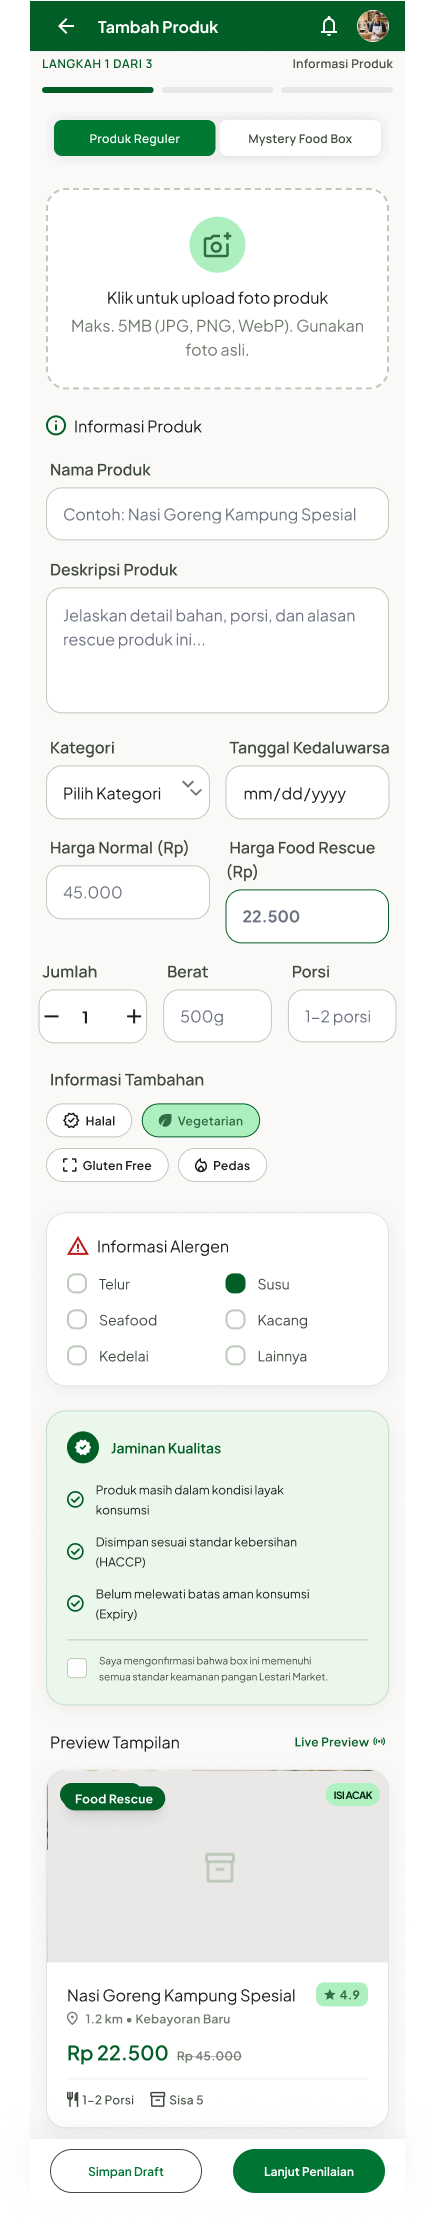
\includegraphics[width=\linewidth, height=6.4cm, keepaspectratio]{gambar/tambah-produk-reguler.png}
\caption{Tambah Produk Reguler}
\label{fig:ui_produk_reguler}
\end{minipage}\hfill
\begin{minipage}[t]{0.49\textwidth}
\centering
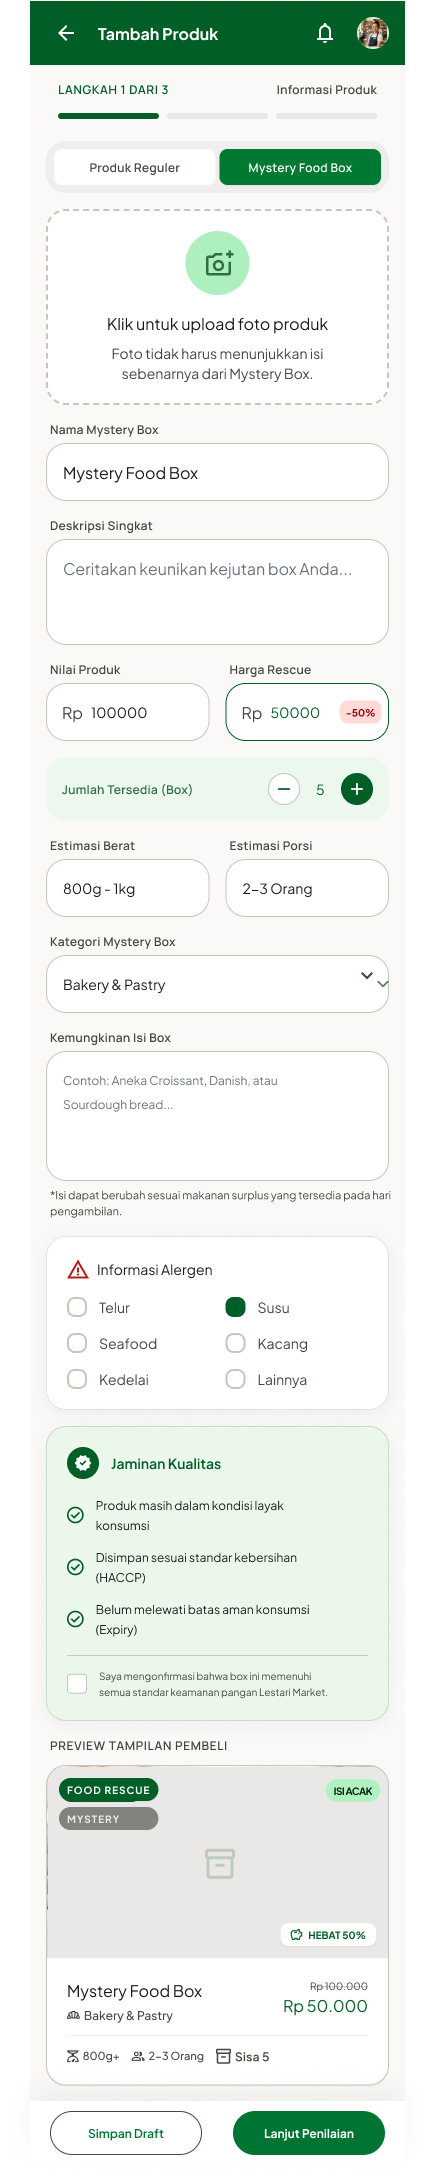
\includegraphics[width=\linewidth, height=6.4cm, keepaspectratio]{gambar/tambah-produk-mysterybox.png}
\caption{Tambah Produk Mystery Box}
\label{fig:ui_produk_mb}
\end{minipage}
\end{figure}

\begin{figure}[htbp]
\centering
\begin{minipage}[t]{0.49\textwidth}
\centering
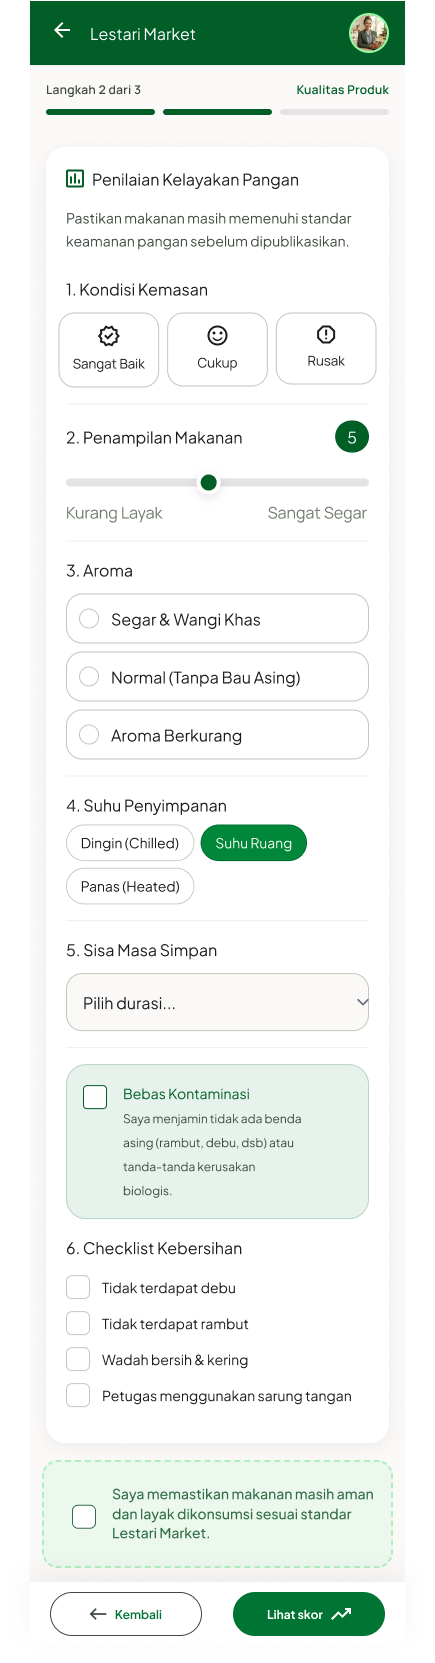
\includegraphics[width=\linewidth, height=6.4cm, keepaspectratio]{gambar/penilaian-kelayakan.png}
\caption{Form Penilaian Kelayakan}
\label{fig:ui_penilaian}
\end{minipage}\hfill
\begin{minipage}[t]{0.49\textwidth}
\centering
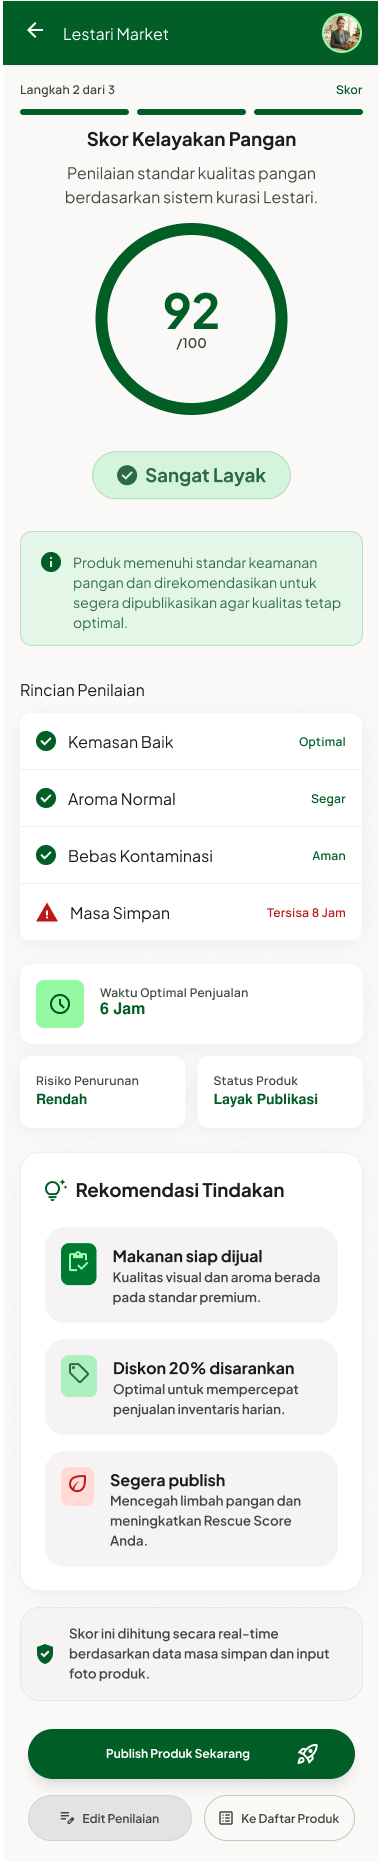
\includegraphics[width=\linewidth, height=6.4cm, keepaspectratio]{gambar/hasil-kelayakan.png}
\caption{Hasil Food Trust Index}
\label{fig:ui_hasil}
\end{minipage}
\end{figure}

\subsubsection{Alur Autentikasi dan Admin (Direncanakan)}

\begin{figure}[htbp]
\centering
\begin{minipage}[t]{0.49\textwidth}
\centering
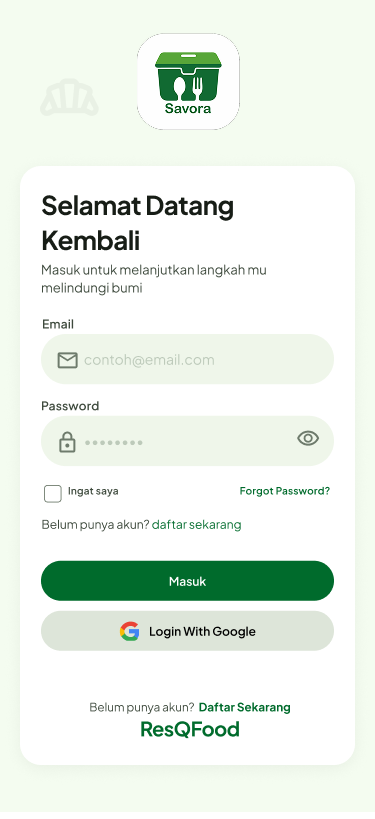
\includegraphics[width=\linewidth, height=6.0cm, keepaspectratio]{gambar/login.png}
\caption{Halaman Login}
\label{fig:ui_login}
\end{minipage}\hfill
\begin{minipage}[t]{0.49\textwidth}
\centering
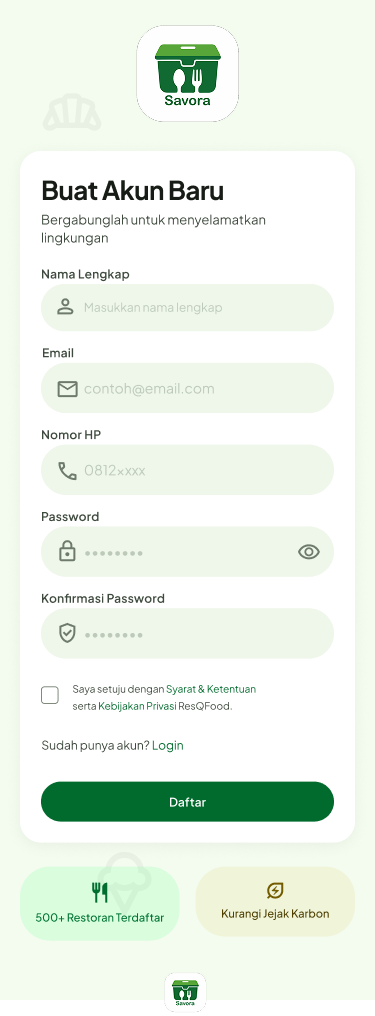
\includegraphics[width=\linewidth, height=6.0cm, keepaspectratio]{gambar/register.png}
\caption{Halaman Register}
\label{fig:ui_register}
\end{minipage}
\end{figure}

\begin{figure}[htbp]
\centering
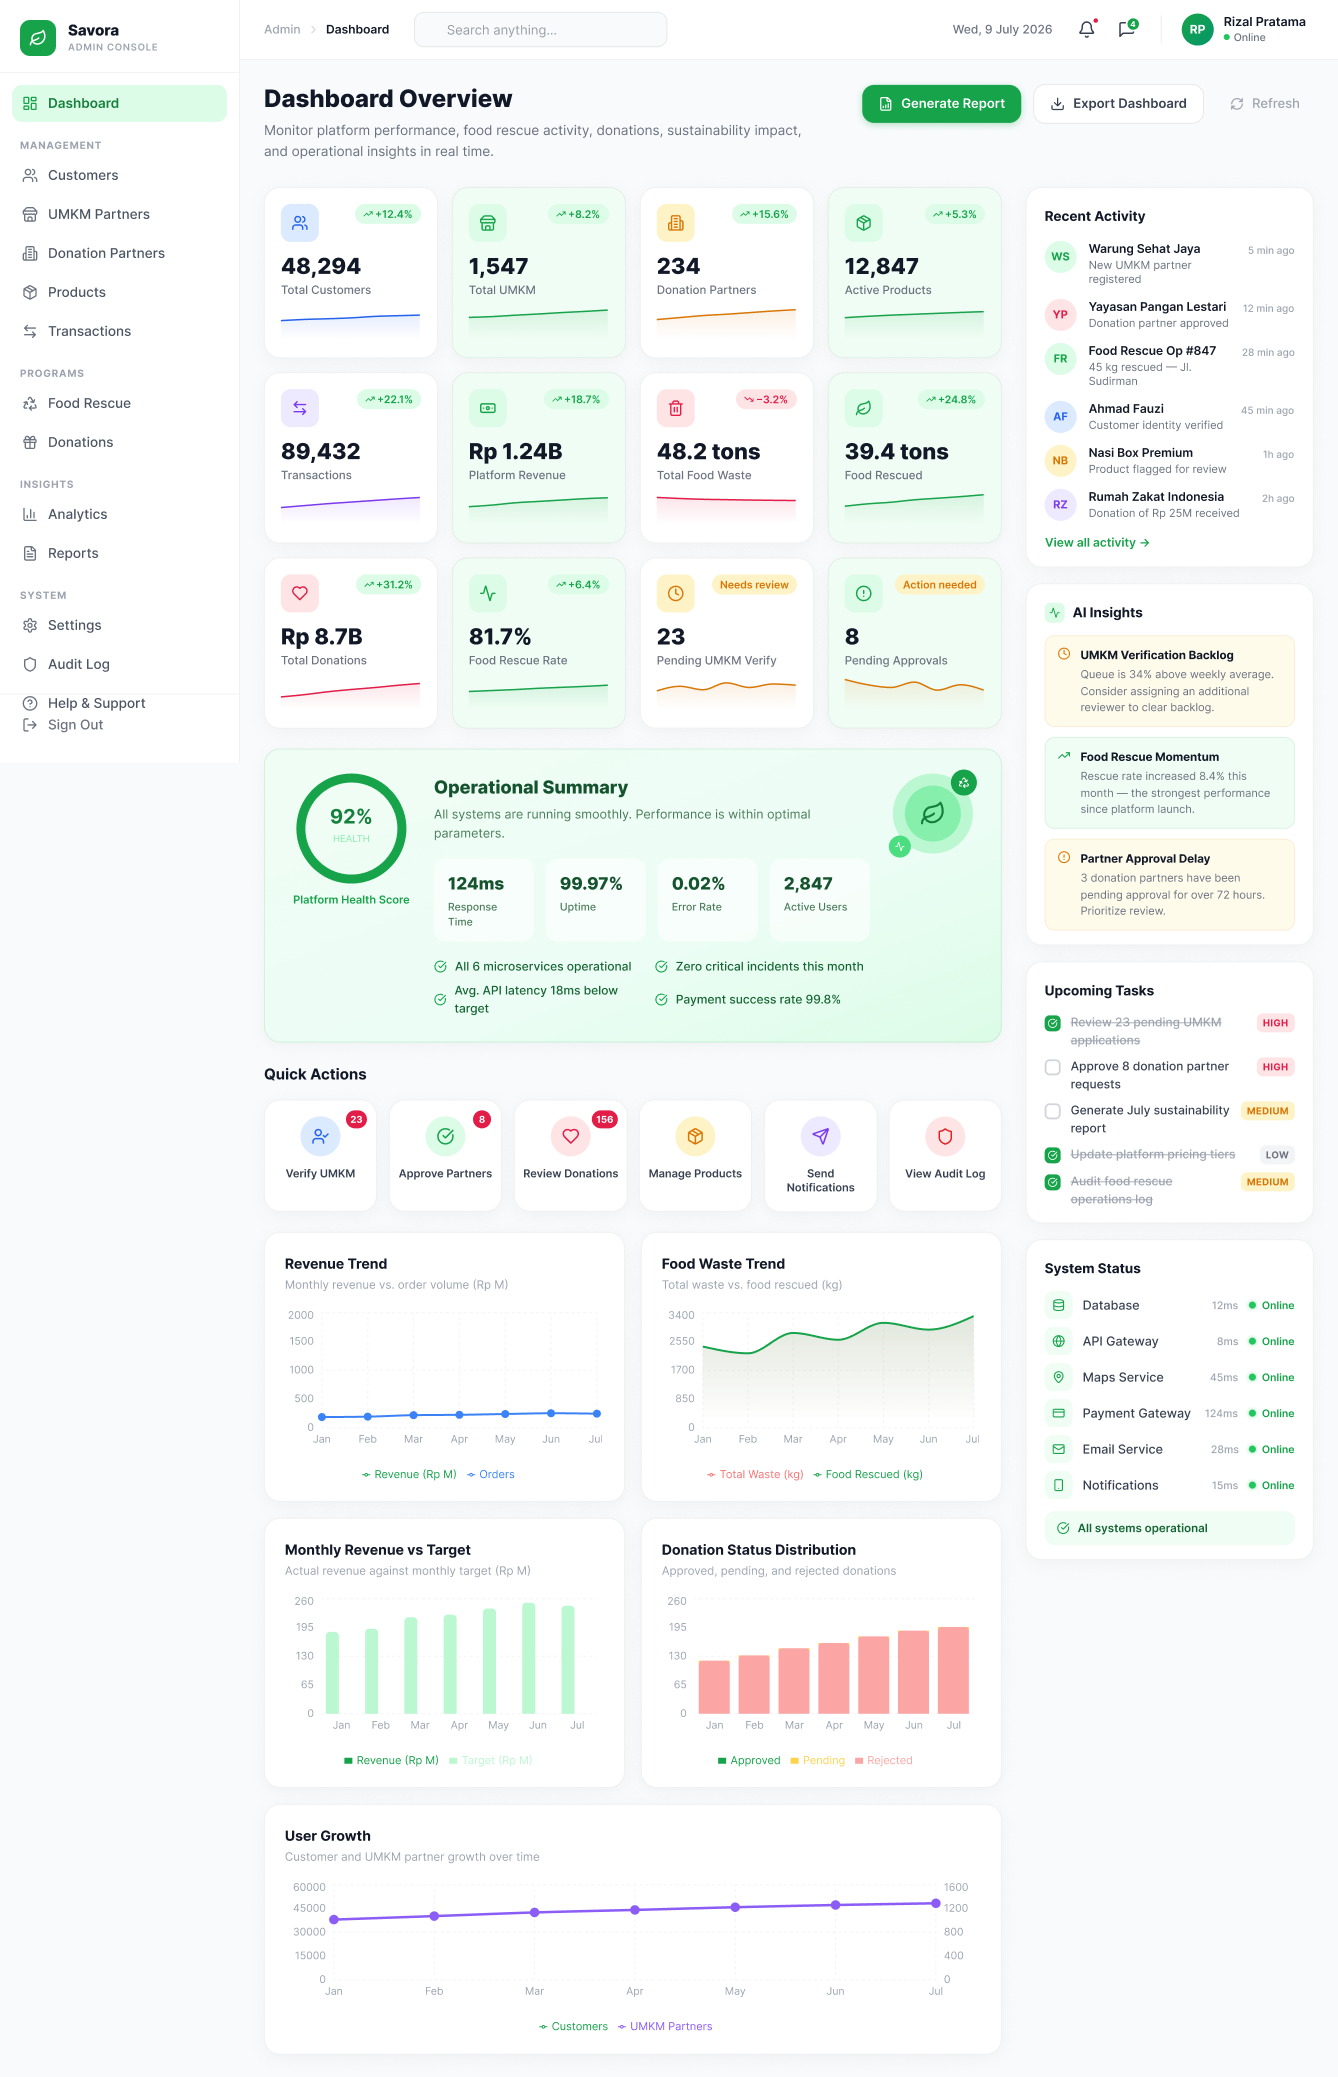
\includegraphics[width=0.74\textwidth, height=6.6cm, keepaspectratio]{gambar/admin-console.png}
\caption{Admin Console (direncanakan)}
\label{fig:ui_admin}
\end{figure}

\subsection{Inventaris Layar MVP}

Tabel~\ref{tab:screens} merangkum layar utama pada rancangan MVP beserta statusnya, agar cakupan
UI selaras dengan ruang lingkup fungsional.

\begin{table}[htbp]
\centering
\caption{Inventaris Layar MVP Savora}
\label{tab:screens}
\small
\begin{tabularx}{\textwidth}{|l|X|l|}
\hline
\textbf{Aktor} & \textbf{Layar} & \textbf{Status} \\
\hline
Customer & Marketplace (Food Score, timer, badge keyword) & Sudah berjalan \\
\cline{2-3}
& Detail produk \& detail UMKM & Sudah berjalan \\
\cline{2-3}
& Checkout cashless + service fee, status \& pickup code & Direncanakan \\
\cline{2-3}
& Help Center (buat tiket) & Direncanakan \\
\hline
UMKM & Dashboard, analitik, insight & Sudah berjalan \\
\cline{2-3}
& Tambah produk (reguler \& mystery box) & Sudah berjalan \\
\cline{2-3}
& Form Food Trust Index \& hasil kelayakan & Sudah berjalan \\
\cline{2-3}
& Validasi pickup code \& Waste Log & Direncanakan \\
\hline
Admin & Verifikasi UMKM \& Mitra Donasi, moderasi & Direncanakan \\
\cline{2-3}
& Dashboard keuangan \& export laporan & Direncanakan \\
\hline
Mitra Donasi & Registrasi \& status verifikasi & Direncanakan \\
\hline
Umum & Login / Register (4 role) & Direncanakan \\
\hline
\end{tabularx}
\end{table}

\subsection{Aksesibilitas dan Prinsip Desain}

Antarmuka Savora dirancang mengikuti prinsip aksesibilitas praktis agar dapat digunakan oleh
rentang pengguna yang luas:

\begin{itemize}[leftmargin=*]
    \item \textbf{Kontras warna} : Status Food Score/rescue timer tidak hanya dibedakan warna
    (merah/kuning/hijau) tetapi juga label teks, agar tetap terbaca oleh pengguna \textit{color-blind}.
    \item \textbf{Target sentuh} : Tombol utama berukuran memadai untuk interaksi \textit{mobile-first}.
    \item \textbf{Teks alternatif} : Gambar produk dan ikon status dilengkapi \textit{alt text}/label.
    \item \textbf{Umpan balik jelas} : Setiap aksi penting (checkout, pembayaran, validasi pickup)
    memberikan konfirmasi status yang eksplisit, sejalan dengan heuristik \textit{visibility of system
    status} \cite{nielsen2020heuristics}.
    \item \textbf{Bahasa sederhana} : Istilah teknis diberi penjelasan singkat, termasuk
    \textit{disclaimer} bahwa Food Trust Index berbasis informasi UMKM.
\end{itemize}

Validasi kepatuhan penuh terhadap WCAG memerlukan pengujian manual dengan teknologi bantu dan
telaah pakar aksesibilitas, yang diposisikan sebagai bagian tahap pengujian lanjutan.

\bigskip

% ==================== BAGIAN 13: PENGUJIAN (TESTING) ====================
\section{RENCANA STRATEGI PENGUJIAN}

\subsection{Strategi Pengujian}

Savora akan menjalani berbagai jenis pengujian untuk memastikan kualitas aplikasi. Berikut adalah rencana testing yang akan diimplementasikan:

\begin{table}[htbp]
\centering
\caption{Jenis Pengujian yang Akan Dilakukan}
\label{tab:testing}
\begin{tabularx}{\textwidth}{|l|X|X|}
\hline
\textbf{Jenis Testing} & \textbf{Deskripsi} & \textbf{Tools yang Akan Digunakan} \\
\hline
Unit Testing & Pengujian fungsi individual & Jest atau Vitest \\
\hline
Integration Testing & Pengujian integrasi antar modul & Jest + Supertest \\
\hline
API Testing & Pengujian endpoint API & Postman atau Supertest \\
\hline
UI Testing & Pengujian antarmuka pengguna & Cypress atau Playwright \\
\hline
Usability Testing & Pengujian kemudahan penggunaan & Manual testing \\
\hline
Performance Testing & Pengujian performa dan beban & Artillery atau k6 \\
\hline
Security Testing & Pengujian keamanan & OWASP ZAP \\
\hline
\end{tabularx}
\end{table}

\textbf{STATUS}: Semua jenis testing di atas adalah RENCANA. Belum ada test yang sudah dibuat atau dijalankan saat ini.

\subsection{Unit Testing (Rencana)}

\subsubsection{Area yang Akan Ditest}
\begin{itemize}[leftmargin=*]
    \item \textbf{Food Trust Index} : Testing pemetaan input UMKM ke lima status kelayakan
    \item \textbf{Food Score Decay} : Testing perhitungan skor peluruhan untuk berbagai sisa waktu
    \item \textbf{Keyword Classification} : Testing pemetaan keyword ulasan ke level Aman/Warning/Gawat dan agregasi \textit{worst-case}
    \item \textbf{Dynamic Discount \& Service Fee} : Testing perhitungan diskon, penghematan, dan \textit{service fee} 5\%
    \item \textbf{Authentication Logic} : Testing login, register, password hashing, RBAC 4 role
    \item \textbf{Data Validation} : Testing validasi input form
\end{itemize}

\subsubsection{Test Coverage Target}
\begin{itemize}[leftmargin=*]
    \item Backend Core Logic (Go): target >80\% coverage
    \item API Routes (Fiber): target >70\% coverage
    \item Logika Food Score \& Pricing (JavaScript): target >75\% coverage
    \item Frontend Components: target >60\% coverage
    \item Overall Project: target >70\% coverage
\end{itemize}

\subsection{Integration Testing (Rencana)}

Akan memastikan komunikasi antar modul berjalan dengan baik:

\begin{itemize}[leftmargin=*]
    \item \textbf{Frontend-Backend Integration} : Memastikan API calls dari frontend berhasil
    \item \textbf{Backend-Database Integration} : Memastikan operasi CRUD via GORM ke PostgreSQL bekerja
    \item \textbf{Food Score Consistency} : Memastikan perhitungan Food Score \& diskon konsisten dengan data produk
    \item \textbf{Payment Integration (Midtrans Sandbox)} : Memastikan pembuatan token, verifikasi \textit{webhook}/\textit{signature}, dan transisi status order (Paid, Failed/Expired) berjalan benar
\end{itemize}

\subsection{API Testing (Rencana)}

Endpoint API akan diuji untuk memastikan response code dan response time optimal:

\begin{table}[htbp]
\centering
\caption{Target API Performance}
\label{tab:api_testing}
\begin{tabularx}{\textwidth}{|l|X|X|}
\hline
\textbf{Endpoint} & \textbf{Expected Status} & \textbf{Target Response Time} \\
\hline
POST /api/auth/register & 201 Created & < 300ms \\
\hline
POST /api/auth/login & 200 OK & < 200ms \\
\hline
GET /api/products & 200 OK & < 150ms \\
\hline
POST /api/products & 201 Created & < 300ms \\
\hline
POST /api/orders & 201 Created & < 400ms \\
\hline
POST /api/payments/midtrans-token & 201 Created & < 500ms \\
\hline
POST /api/payments/midtrans-webhook & 200 OK & < 300ms \\
\hline
PUT /api/orders/:id/status & 200 OK & < 200ms \\
\hline
\end{tabularx}
\end{table}

\subsection{Usability Testing (Rencana)}

Akan dilakukan dengan partisipan yang mewakili target pengguna untuk mengevaluasi:

\begin{enumerate}[leftmargin=*]
    \item \textbf{Learnability} : Seberapa mudah pengguna baru memahami antarmuka
    \item \textbf{Efficiency} : Seberapa cepat pengguna menyelesaikan task
    \item \textbf{Memorability} : Seberapa mudah pengguna mengingat cara penggunaan
    \item \textbf{Errors} : Seberapa sering pengguna melakukan kesalahan
    \item \textbf{Satisfaction} : Seberapa puas pengguna dengan aplikasi
\end{enumerate}

\textbf{Skenario Testing yang Akan Diuji:}

Untuk Customer:
\begin{itemize}[leftmargin=*]
    \item Registrasi akun baru
    \item Mencari produk berdasarkan lokasi
    \item Melihat detail produk, Food Score, dan badge keamanan keyword
    \item Melakukan checkout \textit{cashless} via Midtrans (sandbox) dengan \textit{service fee} 5\%
    \item Memantau status pesanan dan menunjukkan \textit{pickup code}
    \item Memberikan rating dan review (termasuk keyword)
    \item Membuat tiket di Help Center
\end{itemize}

Untuk UMKM:
\begin{itemize}[leftmargin=*]
    \item Registrasi dan verifikasi akun
    \item Menambahkan produk surplus, mengisi Food Trust Index, dan menetapkan harga rescue
    \item Memantau Food Score produk
    \item Memvalidasi \textit{pickup code} dan memproses pesanan
    \item Mencatat Waste Log dan melihat analitik/insight
\end{itemize}

Untuk Admin dan Mitra Donasi:
\begin{itemize}[leftmargin=*]
    \item Admin memverifikasi UMKM dan Mitra Donasi (approve/reject)
    \item Admin memoderasi iklan dan menangani Help Ticket
    \item Admin melihat dashboard keuangan dan meng-\textit{export} laporan
    \item Mitra Donasi mendaftar dan memantau status verifikasi
\end{itemize}

\subsection{Performance Testing (Rencana)}

Akan mensimulasikan beban pengguna untuk memastikan aplikasi dapat handle traffic tinggi:

\begin{table}[htbp]
\centering
\caption{Target Metrik Performa}
\label{tab:performance}
\begin{tabularx}{\textwidth}{|l|X|X|}
\hline
\textbf{Metrik} & \textbf{Target} & \textbf{Kondisi} \\
\hline
Response Time (rata-rata) & < 500ms & Load normal \\
\hline
Response Time (p95) & < 1000ms & Load normal \\
\hline
Concurrent Users & 100+ & Tanpa degradasi performa \\
\hline
Throughput & 50+ req/sec & Per endpoint \\
\hline
Error Rate & < 1\% & Semua kondisi \\
\hline
\end{tabularx}
\end{table}

\textbf{Load Testing Scenarios yang Akan Dilakukan:}
\begin{itemize}[leftmargin=*]
    \item Normal Load: 50 concurrent users selama 10 menit
    \item Peak Load: 100 concurrent users selama 5 menit
    \item Stress Test: Gradually increase users hingga sistem menunjukkan degradasi
    \item Spike Test: Sudden increase dari 10 ke 100 users dalam 30 detik
\end{itemize}

\subsection{Security Testing (Rencana)}

Akan fokus pada OWASP Top 10 vulnerabilities:

\begin{enumerate}[leftmargin=*]
    \item \textbf{SQL Injection} : Memastikan input user di-sanitize dengan ORM
    \item \textbf{Authentication} : Memastikan password di-hash, token JWT secure
    \item \textbf{XSS Protection} : Memastikan user input di-escape
    \item \textbf{CSRF Protection} : Implementasi CSRF token untuk forms
    \item \textbf{Sensitive Data} : Memastikan password tidak di-log atau exposed
    \item \textbf{API Security} : Implementasi rate limiting dan CORS policy
\end{enumerate}

\subsection{Kriteria Penerimaan (Acceptance Criteria)}

Tabel~\ref{tab:acceptance} merangkum kriteria penerimaan fitur inti MVP yang menjadi dasar
verifikasi \textit{end-to-end} saat demo.

\begin{table}[htbp]
\centering
\caption{Kriteria Penerimaan Fitur Inti MVP}
\label{tab:acceptance}
\small
\begin{tabularx}{\textwidth}{|l|X|}
\hline
\textbf{Fitur} & \textbf{Kriteria Penerimaan} \\
\hline
Food Trust Index & Input UMKM menghasilkan salah satu dari 5 status; produk berstatus tidak layak tidak tampil di marketplace \\
\hline
Food Score Decay & Skor menurun mengikuti sisa waktu dan mencapai 0 saat kedaluwarsa; label band sesuai ambang \\
\hline
Keyword Classification & Ulasan dengan keyword gawat menaikkan badge UMKM ke level terburuk (worst-case) \\
\hline
Checkout Cashless & Total = subtotal + service fee 5\%; status menjadi Paid hanya setelah verifikasi notifikasi Midtrans \\
\hline
Pickup Code & Kode unik terbentuk setelah Paid; order menjadi Completed hanya jika kode valid \\
\hline
Help Center & Tiket customer tersimpan dan tampil di konsol admin untuk ditindaklanjuti \\
\hline
Waste Log & Catatan makanan tidak terjual tersimpan dan terlihat pada dashboard UMKM \\
\hline
Mitra Donasi & Registrasi berstatus pending; berubah aktif hanya setelah admin melakukan approve \\
\hline
Keuangan Admin & Total service fee + iklan tercatat dan dapat di-export (CSV/Excel/PDF) \\
\hline
\end{tabularx}
\end{table}

\subsection{Testing Timeline}

\begin{table}[htbp]
\centering
\caption{Rencana Timeline Pengujian}
\label{tab:testing_timeline}
\begin{tabularx}{\textwidth}{|l|X|l|}
\hline
\textbf{Fase} & \textbf{Aktivitas} & \textbf{Durasi} \\
\hline
Development & Unit testing parallel dengan development & Ongoing \\
\hline
Integration & Integration testing setelah modul selesai & 1 minggu \\
\hline
System Testing & API, UI, performance testing & 1-2 minggu \\
\hline
User Acceptance & Usability testing dengan target user & 1 minggu \\
\hline
Security & Security audit dan penetration testing & 1 minggu \\
\hline
\end{tabularx}
\end{table}

\subsection{Bug Tracking dan Issue Management}

Untuk mengelola bug dan issue yang ditemukan:

\begin{itemize}[leftmargin=*]
    \item \textbf{Platform} : GitHub Issues untuk tracking
    \item \textbf{Priority Levels} : Critical, High, Medium, Low
    \item \textbf{Bug Report Template} : Steps to reproduce, expected vs actual behavior
    \item \textbf{Definition of Done} : Bug fix must include test case
\end{itemize}

\subsection{Continuous Integration (Rencana)}

Testing akan diintegrasikan dengan CI/CD pipeline:

\begin{itemize}[leftmargin=*]
    \item \textbf{Pre-commit Hooks} : Linting dan formatting check
    \item \textbf{Pull Request Checks} : Unit tests dan integration tests otomatis
    \item \textbf{Code Coverage Report} : Automated coverage report di setiap PR
    \item \textbf{Security Scan} : Dependency vulnerability check
\end{itemize}

\textbf{CATATAN PENTING}: Semua rencana testing di atas akan diimplementasikan pada fase development. Saat ini belum ada test yang sudah ditulis atau dijalankan. Aplikasi belum dibangun sehingga tidak ada hasil testing yang dapat dilaporkan.

\bigskip

% ==================== BAGIAN 14: DOKUMENTASI PENGGUNAAN ====================
\section{RENCANA DOKUMENTASI DAN DEPLOYMENT}

\subsection{Rencana Deployment}

Savora akan di-deploy menggunakan strategi berikut setelah development selesai:

\begin{enumerate}[leftmargin=*]
    \item \textbf{Frontend} : Deployment ke platform seperti Vercel atau Netlify dengan continuous deployment dari GitHub
    \item \textbf{Backend} : Deployment ke cloud provider seperti Railway, Render, atau AWS dengan auto-scaling capability
    \item \textbf{Database} : PostgreSQL managed instance (Supabase, Railway, atau AWS RDS)
    \item \textbf{Backend Runtime} : Biner Go dikemas dalam Docker container untuk portabilitas
\end{enumerate}

\textbf{STATUS}: Deployment belum dilakukan. Aplikasi masih dalam tahap perencanaan dan akan di-deploy setelah development selesai.

\subsection{Rencana Dokumentasi Pengguna}

Dokumentasi akan dibuat untuk memudahkan pengguna menggunakan aplikasi setelah deployment:

\subsubsection{User Guide untuk Customer}
Akan mencakup:
\begin{itemize}[leftmargin=*]
    \item Cara registrasi dan login
    \item Cara mencari produk dan membaca badge keamanan keyword
    \item Cara memahami Food Score dan rescue timer
    \item Cara checkout \textit{cashless} via Midtrans dan menggunakan \textit{pickup code}
    \item Cara tracking pesanan
    \item Cara memberikan review dan membuat tiket Help Center
    \item Cara melihat impact dashboard
\end{itemize}

\subsubsection{User Guide untuk UMKM}
Akan mencakup:
\begin{itemize}[leftmargin=*]
    \item Cara registrasi dan verifikasi
    \item Cara menambahkan produk dan mengisi Food Trust Index
    \item Cara memahami Food Score produk
    \item Cara menetapkan harga rescue (time-aware pricing)
    \item Cara memvalidasi \textit{pickup code} dan mengelola pesanan
    \item Cara mencatat Waste Log dan membaca analitik/insight
\end{itemize}

\subsubsection{User Guide untuk Admin}
Akan mencakup:
\begin{itemize}[leftmargin=*]
    \item Cara mengakses admin panel
    \item Cara verifikasi UMKM dan Mitra Donasi baru
    \item Cara monitoring platform dan dashboard keuangan (service fee + iklan)
    \item Cara moderasi konten/iklan dan menangani Help Ticket
    \item Cara meng-\textit{export} laporan (CSV/Excel/PDF)
\end{itemize}

\subsubsection{User Guide untuk Mitra Donasi}
Akan mencakup:
\begin{itemize}[leftmargin=*]
    \item Cara registrasi organisasi dan mengunggah dokumen legalitas
    \item Cara memantau status verifikasi
    \item Cara menerima informasi makanan surplus
\end{itemize}

\subsection{Rencana Akun Demo}

Untuk keperluan testing dan penilaian kompetisi, akan disediakan akun demo:

\begin{table}[htbp]
\centering
\caption{Rencana Akun Demo}
\label{tab:akun_demo}
\begin{tabularx}{\textwidth}{|l|X|X|}
\hline
\textbf{Role} & \textbf{Email} & \textbf{Purpose} \\
\hline
Admin & admin@savora.demo & Testing fitur admin, verifikasi, keuangan \\
\hline
UMKM & umkm@savora.demo & Testing workflow UMKM \& Food Trust Index \\
\hline
Customer & customer@savora.demo & Testing alur belanja \& checkout cashless \\
\hline
Mitra Donasi & mitra@savora.demo & Testing registrasi \& verifikasi mitra donasi \\
\hline
\end{tabularx}
\end{table}

\textbf{Sample Data yang Akan Di-seed:}
\begin{itemize}[leftmargin=*]
    \item 10+ UMKM dengan profil lengkap
    \item 30+ produk makanan surplus dengan berbagai kategori
    \item 50+ transaksi historis untuk testing
    \item Review dan rating dari customer
    \item Statistik dashboard (food waste saved, carbon impact)
\end{itemize}

\textbf{CATATAN}: Akun demo dan sample data di atas adalah RENCANA. Belum ada aplikasi yang di-deploy saat ini.

\subsubsection{Pembayaran Demo (Midtrans Sandbox)}

Karena pembayaran menggunakan Midtrans mode \textit{sandbox}, tidak ada uang asli yang berpindah.
Untuk demo dan penilaian, checkout dapat diselesaikan menggunakan kredensial uji Midtrans (mis.
kartu uji dan simulator \textit{e-wallet}/VA yang disediakan Midtrans). Alur demo pembayaran:

\begin{enumerate}[leftmargin=*]
    \item Customer memilih produk dan menekan \textit{checkout}; sistem menampilkan subtotal,
    \textit{service fee} 5\%, dan total.
    \item Sistem membuat transaksi ke Midtrans \textit{sandbox} dan menampilkan halaman pembayaran.
    \item Penilai menyelesaikan pembayaran dengan kredensial uji Midtrans.
    \item Midtrans mengirim notifikasi; setelah diverifikasi, status order menjadi \emph{Paid} dan
    \textit{pickup code} dibuat.
    \item UMKM memvalidasi \textit{pickup code} untuk menyelesaikan pesanan.
\end{enumerate}

\textbf{CATATAN}: Kredensial kartu/uji Midtrans akan disertakan pada README repositori, bukan
dituliskan di proposal, dan hanya berlaku pada lingkungan \textit{sandbox}.

\subsection{Requirement Sistem}

Aplikasi Savora akan memiliki requirement minimum berikut:

\begin{table}[htbp]
\centering
\caption{Minimum System Requirements}
\label{tab:requirements}
\begin{tabularx}{\textwidth}{|l|X|}
\hline
\textbf{Komponen} & \textbf{Spesifikasi Minimum} \\
\hline
Browser & Chrome 90+, Firefox 88+, Safari 14+, Edge 90+ \\
\hline
Koneksi Internet & 2 Mbps untuk pengalaman optimal \\
\hline
Device & Desktop, laptop, tablet, atau smartphone \\
\hline
Screen Resolution & 360px width minimum (mobile-first) \\
\hline
JavaScript & Enabled (required) \\
\hline
\end{tabularx}
\end{table}

\subsection{Rencana FAQ dan Troubleshooting}

Dokumentasi FAQ dan troubleshooting akan dibuat mencakup:

\subsubsection{Common Issues yang Akan Didokumentasikan}
\begin{itemize}[leftmargin=*]
    \item Masalah login dan authentication
    \item Masalah loading halaman
    \item Masalah upload gambar
    \item Masalah pembayaran Midtrans (sandbox) dan status order
    \item Masalah notifikasi
    \item Masalah perhitungan Food Trust Index / Food Score
\end{itemize}

Setiap issue akan didokumentasikan dengan:
\begin{enumerate}[leftmargin=*]
    \item Deskripsi masalah
    \item Penyebab umum
    \item Langkah-langkah solusi
    \item Cara menghubungi support jika tidak terselesaikan
\end{enumerate}

\subsection{Rencana Support dan Kontak}

Setelah deployment, akan tersedia channel support:

\begin{itemize}[leftmargin=*]
    \item \textbf{Email Support} : Untuk pertanyaan dan issue teknis
    \item \textbf{GitHub Issues} : Untuk bug reports dan feature requests
    \item \textbf{Documentation Website} : Knowledge base dan tutorials
\end{itemize}

\subsection{Dokumentasi Teknis untuk Developer}

Akan dibuat dokumentasi teknis mencakup:

\subsubsection{API Documentation}
\begin{itemize}[leftmargin=*]
    \item Daftar semua endpoints dengan method dan parameters
    \item Request/response examples
    \item Authentication requirements
    \item Error codes dan handling
    \item Rate limiting policies
\end{itemize}

\subsubsection{Database Schema Documentation}
\begin{itemize}[leftmargin=*]
    \item Entity Relationship Diagram (ERD)
    \item Table descriptions
    \item Field definitions dan constraints
    \item Relationships dan foreign keys
    \item Indexes dan performance considerations
\end{itemize}

\subsubsection{Deployment Guide}
\begin{itemize}[leftmargin=*]
    \item Environment setup instructions
    \item Configuration requirements
    \item Database migration steps
    \item CI/CD pipeline setup
    \item Monitoring dan logging setup
\end{itemize}

\subsection{Rencana Maintenance Documentation}

Dokumentasi maintenance akan mencakup:

\begin{itemize}[leftmargin=*]
    \item \textbf{Backup Strategy} : Frequency, retention policy, restore procedures
    \item \textbf{Monitoring} : Key metrics to track, alerting thresholds
    \item \textbf{Scaling Guidelines} : When and how to scale infrastructure
    \item \textbf{Security Updates} : Process for patching vulnerabilities
    \item \textbf{Performance Optimization} : Common bottlenecks dan solutions
\end{itemize}

\subsection{Timeline Dokumentasi}

\begin{table}[htbp]
\centering
\caption{Rencana Timeline Dokumentasi}
\label{tab:doc_timeline}
\begin{tabularx}{\textwidth}{|l|X|l|}
\hline
\textbf{Fase} & \textbf{Deliverable} & \textbf{Timing} \\
\hline
Development & API documentation, code comments & Ongoing \\
\hline
Pre-deployment & User guides, admin documentation & 1-2 minggu \\
\hline
Post-deployment & FAQ, troubleshooting guide & Iteratif \\
\hline
Maintenance & Technical documentation updates & Ongoing \\
\hline
\end{tabularx}
\end{table}

\textbf{CATATAN PENTING}: Semua dokumentasi di atas adalah RENCANA yang akan dibuat setelah aplikasi selesai dibangun dan di-deploy. Saat ini aplikasi belum ada, sehingga belum ada user guide, FAQ, atau troubleshooting documentation yang dapat diberikan. Dokumentasi akan dibuat bertahap seiring dengan progress development dan feedback dari user testing.

\clearpage

% ==================== BAGIAN 15: DAFTAR PUSTAKA & REFERENSI ====================
\section*{DAFTAR PUSTAKA \& REFERENSI}
\phantomsection
\addcontentsline{toc}{section}{DAFTAR PUSTAKA \& REFERENSI}
% Biblatex Automated Bibliography dengan IEEE Numeric Hyperlinks
\printbibliography[heading=none]

\clearpage

% ==================== LAMPIRAN ====================
% Lampiran A (skema DB kolom-per-kolom) dihapus: struktur data sudah dirangkum
% pada Tabel "Struktur Data Model Savora" di BAB Arsitektur Sistem (bab8),
% sekaligus menjaga konsistensi istilah (food_score, service_fee, rescue_price).

\end{document}
